\documentclass{tudelft-report}
\usepackage{natbib}
\usepackage{changes}
\usepackage{amsthm}
\usepackage{float}
\usepackage{subcaption}
\usepackage{graphicx}

\begin{document}

%% Use Roman numerals for the page numbers of the title pages and table of
%% contents.
\frontmatter

%% Uncomment following 19 lines for a cover with a picture on the lower half only
% \title[tudelft-white]{Title}
% \subtitle[tudelft-cyan]{Optional subtitle}
% \author[tudelft-white]{J.\ Random Author}
% \affiliation{Technische Universiteit Delft}
% \coverimage{cover.jpg}
% \titleoffsetx{10cm}
% \titleoffsety{10cm}
% \afiloffsetx{1cm}
% \afiloffsety{18cm}
% \covertext[tudelft-white]{
%    \textbf{Cover Text} \\
%    possibly \\
%    spanning 
%    multiple 
%    lines
%    \vfill
%    ISBN 000-00-0000-000-0
% }
% \makecover

% Uncomment following 16 lines for a cover with a picture on the lower half only
\title[tudelft-white]{The Optimal\\Transport\\Problem}
\subtitle[tudelft-white]{Master Thesis}
\author[tudelft-white]{Oscar Ramirez}
\affiliation{Msc. in Mathematical modelling in Engineering.}
\coverimage{Barcelona2.jpg}
\covertext[tudelft-white]{
%    \textbf{Cover Text} \\
%    possibly \\
%    spanning 
%    multiple 
%    lines
%    \vfill
%    ISBN 000-00-0000-000-0
}
\setpagecolor{tudelft-blue}
\makecover[split, whitelogo]

\graphicspath{{./Pictures/}}
%% Include an optional title page.
\begin{titlepage}


\begin{center}

%% Insert the TU Delft logo at the bottom of the page.

%% Print the title in cyan.
{\makeatletter
\largetitlestyle\fontsize{64}{94}\selectfont\@title
%\largetitlestyle\color{tudelft-cyan}\Huge\@title
\makeatother}

%% Print the optional subtitle in black.
{\makeatletter
\ifx\@subtitle\undefined\else
    \bigskip
   {\tudsffamily\fontsize{22}{32}\selectfont\@subtitle}    
    %\titlefont\titleshape\LARGE\@subtitle
\fi
\makeatother}

\bigskip
\bigskip

by
%door

\bigskip
\bigskip

%% Print the name of the author.
{\makeatletter
%\largetitlefont\Large\bfseries\@author
\largetitlestyle\fontsize{26}{26}\selectfont\@author
\makeatother}

\bigskip
\bigskip

to obtain the degree of Master of Science
%ter verkrijging van de graad van Master of Science

in Mathematical Modelling and Engineering,
%aan de Technische Universiteit Delft,

to be defended publicly on September, 2018.
%in het openbaar de verdedigen op dinsdag 1 januari om 10:00 uur.

\vfill

\begin{tabular}{lll}
%    Student number: & 1234567 \\
    Project duration: & \multicolumn{2}{l}{September, 2016 -- September, 2018}\\
    Thesis committee: & Prof. Juan Enrique Martinez Legaz, & UAB, supervisor \\
%        & Dr.\ E.\ L.\ Brown, & TU Delft \\
%        & Ir.\ A.\ Aaronson, & Acme Corporation
\end{tabular}
%% Only include the following lines if confidentiality is applicable.

\bigskip
\bigskip
%\emph{This thesis is confidential and cannot be made public until December 31, 2013.}
%\emph{Op dit verslag is geheimhouding van toepassing tot en met 31 december 2013.}

%\bigskip
%\bigskip
%An electronic version of this thesis is available at \url{http://repository.tudelft.nl/}.
%\\[1cm]

%\centering{
\includegraphics{cover/logo_black}}


\end{center}

\begin{tikzpicture}[remember picture, overlay]
    \node at (current page.south)[anchor=south,inner sep=0pt]{
        
\includegraphics{cover/logo}
    };
\end{tikzpicture}
\bigskip
\bigskip
\end{titlepage}



\chapter*{Preface}
\setheader{Preface}

The optimal transport problem was proposed by Gaspard Monge in 1781. Monge was interested in finding a way to transport a fixed amount of sand from one place into another, without losing or gaining mass in the process, such that the transportation cost is optimal. Later, Leonid Kantorovich introduced the proper framework to understand the problem in terms of probability measures, instead of using maps as Monge proposed the first time. The following work is a brief review of the theory developed for this problem, computation of a solution for a discrete optimal transport problem and two results of the developed theory that can be used in applications. 

The literature in this topic is really rich and researchers in empirical sciences (such as economy, physics, meteorology, among many others) have found connection between the optimal transport problem and problems related to their respective branches, that at first glance seem disconnected from the transportation problem. 

We have divided this text into five chapters. The first one is a reminder about concepts in topology, functional analysis, convex analysis and convergence of probability measures. These concepts are used to find the conditions that assure the existence of a minimizer for the optimal transport problem. If the reader is already familiarized with these concepts please skip directly to the third chapter. The second chapter is a reminder on important results in Linear programming, they are useful to compute a solution for the discrete version of the problem. In case the reader is already familiarized with linear programming, please skip directly to the fourth chapter. The third chapter is the heart of the text, it introduces the problem and we do a brief summary of th theory developed for the problem. The fourth chapter presents the algorithms used to compute a solution for a discrete version of the optimal transport. Finally, in the fifth chapter we discuss how the theory can be used as statistical distance between two probability measures, and an example of how a data assimilation problem can be also seen as an optimal transport problem.

\begin{flushright}
{\makeatletter\itshape
    \@author \\
    Barcelona, September 2018
\makeatother}
\end{flushright}


\newcommand{\ubar}[1]{\underaccent{\bar}{#1}}
\newcommand{\asterisk}[1]{{#1}^*}
\newcommand{\law}{\mathrm{law}}
\newcommand{\dx}{\mathrm{dx}}
\newcommand{\dy}{\mathrm{dy}}
\newcommand{\dmu}{\mathrm{d}\mu}
\newcommand{\dnu}{\mathrm{d}\nu}
\newcommand{\spt}{\mathrm{spt}}
\newcommand{\subject}{\text{subject to }}
\newcommand{\Lebesgue}{\mathcal{L}}
\newcommand{\Hausdorff}{\mathcal{H}}
\newcommand{\weakconvergence}{\rightharpoonup}
\newcommand{\otherwise}{\text{otherwise}}
\newcommand{\Real}{\mathbb{R}}
\newcommand{\Realex}{\bar{\mathbb{R}}}
\newcommand{\Complex}{\mathbb{C}}
\newcommand{\Naturals}{\mathbb{N}}
\newcommand{\X}{\mathcal{X}}
\newcommand{\Y}{\mathcal{Y}}
\newcommand{\braces}[1]{\left\lbrace #1 \right\rbrace}
\newcommand{\brackets}[1]{\left[ #1 \right]}
\newcommand{\parentheses}[1]{\left( #1 \right)}
\newcommand{\anglesbox}[1]{\left\langle #1 \right\rangle}

\newtheorem{theorem}{Theorem}
\newtheorem{problem}{Problem}
\newtheorem{definition}{Definition}
\newtheorem{proposition}{Proposition}
\newtheorem{lemma}{Lemma}
\newtheorem{corollary}{Corollary}
\newcommand{\PlanSp}{\mathcal{P}}
\newcommand{\MeasureSp}{\mathcal{M}}
\newcommand{\PMeasureSp}{\mathcal{M}_+}
\newcommand{\Kantorovich}{K\left(\gamma\right)}
\newcommand{\Monge}{M\left(T\right)}
\newcommand{\TransPlansSet}[2]{\Pi\left(#1, #2\right)}
\newcommand{\WassersteinSp}[1]{\mathbb{W}_{#1}}
\newcommand{\WassersteinDist}[1]{W_{#1}}
\newcommand{\DualTransport}{DP\parentheses{\phi, \psi}}

\newcommand{\indicator}[1]{\mathbb{1}_#1}
\newcommand{\Tmeasure}[2]{{#2}_{\#} #1}
\newcommand{\measurerestr}{%
	\,\raisebox{-.127ex}{\reflectbox{\rotatebox[origin=br]{-90}{$\lnot$}}}\,%
}

\newcommand{\mand}{%
	\mathrm{and}
}


\newcommand{\domainrestr}[2]{{#2}_{\left| #1 \right.}}
\newcommand{\Variation}[2]{ \frac{\delta #1}{\delta #2}}
\newcommand{\dev}[1]{\frac{\mathrm{d}}{\mathrm{d}#1}}
\newcommand{\diff}{\mathrm{d}}
\newcommand{\id}{\mathrm{id}}
\newcommand{\D}{\mathrm{D}}
\tableofcontents

%% Use Arabic numerals for the page numbers of the chapters.
\mainmatter

\chapter{Preliminaries.}
\section{Notation}
\begin{tabular}{ l l }
	$\Real$ & Real numbers field. \\ 
	$\Realex$ & $ \Real \cup \braces{+\infty}$. That is $[-\infty, \infty]$ \\
	$\Real_+ $ & The set of nonnegative real numbers, that is the interval $[0, \infty)$.\\
	$\Realex_+$ & The set of nonnegative extended real numbers, that is the interval $[0, \infty]$\\
	$\delta_x$ & The Dirac mass at point x. \\
	$\Real^d $ & The $d$-dimensional Euclidean space.\\
	$\id$ & Identity map.\\
	$\PlanSp\parentheses{X}$ & Space of probabilities on $X$. \\	
	$\mu \ll\nu$ & The measure is absolutely continuous with respect to $\nu$. \\
	$\indicator{\Omega} $ & Indicator function of a set $\Omega$. If $x\in \Omega$ then $\indicator{\Omega}(x)=1$. If $x\in \Omega^c$, we have $\indicator{\Omega}(x)=0$.\\
	$\mu \measurerestr A$ & A measure $\mu$ restricted to a set $A$.\\
	$\omega_d$ & The Measure of the unite ball in $\Real^d$. \\
	$\wedge$ & The min operator, that is $a\wedge b:=\min\braces{a,b}$. \\
	$\vee$ & The max operator, that is $a\vee b:=\max\braces{a,b}$. \\
	$\D T(x)$ & Jacobian matrix of a map $T(x)$. \\
	$\Tmeasure{\mu}{T}$ &  The image measure of $\mu$ through the map $T$.\\
	$\domainrestr{\Omega}{f}$ & The restriction of a function $f$ to a set $\Omega$. \\
	$\TransPlansSet{\mu}{\nu}$ & The set of transport plans from $\mu$ to $\nu$.\\
	$\Variation{F}{\rho}$ &  First variation of $F:\PlanSp\parentheses{X} \rightarrow \Real$, that is $\left.\dev{\epsilon}F\left(\rho +\epsilon\chi\right)\right|_{\epsilon=0}=\int\Variation{F}{\rho}\diff\chi$\\
	$\WassersteinDist{p}$ & Wasserstein distance of order $p$. \\	
	$\WassersteinSp{p}$ & Wasserstein space of order $p$.\\
 	$\gamma_T$ & The transport plan in $\TransPlansSet{\mu}{\nu}$ induced by a map $T$. That is $\gamma_T = (\id, T)_\#\mu$ and $T_\#\mu=\nu$. \\
	$\Monge$ & Monge cost of a map $T$. \\
	$\Kantorovich$ & Kantorovich cost of a plan $\gamma$. \\	
	$\mu \otimes \nu$ & The product measure of $\mu$ and $\nu$ such that $\mu \otimes \nu (A\times B)= \mu(A)\nu(B)$.\\
	$M^{k\times h}$ & The set of real matrices with $k$ rows and $h$ columns. \\
	$M^\top$ & Transpose of a matrix $M$. \\
	i.i.d. & Independent and identical probability distributions.\\
	l.s.c. & Lower semicontinuous.
\end{tabular}



\section{Definitions and important theorems to remember.}

We start this chapter reminding the basic definitions in topology and measure theory.
\begin{definition}[]
\end{definition}


\begin{definition}
	Let $X$ be a Hausdorff space. Let $\mathcal{V}(x_0)$ be a topological basis of $X$, such that all $V\in \mathcal{V}$ contains $x_0$. Let $f: X\rightarrow \Realex$ a functional valued in $\Realex$. We define, 
	\begin{equation*}
	\liminf_{x\rightarrow x_0} f(x)= \sup_{V\in \mathcal{V}(x_0)} \inf_{s\in V}\ f(s)
	\end{equation*}
	\begin{equation*}
	\limsup_{x\rightarrow x_0} f(x)= \inf_{V\in \mathcal{V}(x_0)} \sup_{s\in V}\ f(s)
	\end{equation*}
	
The above definitions can be expressed in terms of sequences of real numbers. Let $(x_n)_{n \in \Naturals}$ be a sequence in $X$, the above formulation is equivalent to say.
\begin{equation*}
	\liminf_{n\in \Naturals} x_n := \lim_{n\rightarrow \infty} \parentheses{\inf_{m\geq n} x_m}
\end{equation*}
Equivalently for $\limsup$,
	\begin{equation*}
	\liminf_{n\in \Naturals} x_n := \lim_{n\rightarrow \infty} \parentheses{\sup_{m\geq n} x_m}
	\end{equation*}

Please note that the convergence to some point $x_0$, $(x_n)_{n\in \Naturals}\rightarrow x_0$ is not required in the last definitions.
\end{definition}

\begin{definition}[Lower Semicontinuity]
	On a complete metric space $X$, a function $f: X\rightarrow\Realex$ is said to be lower semi-continuous (l.s.c.) if for every sequence $\parentheses{x_n}_{n\in\Naturals}$ converging to $x\in X$, we have \begin{equation*}
		f(x)\leq \liminf_{n\in \Naturals} f(x_n)
	\end{equation*}
\end{definition}

\begin{definition}[Sequentially compact]
	A subset $K$ of a metric space $X$ is said to be compact if from any sequence $x_n$, we can extract a converging subsequence $x_{n_k} \rightarrow x \in K$.
\end{definition}
We can see from the above definition that any continuous function is lower-semicontinuous. 

\begin{definition}[Compactness]
		A subset $K$ of a metric space $X$ is compact if every open cover of $K$ has a finite subcover. 
\end{definition}

\begin{theorem}
	A subset of a metric space is compact if and only if it is sequentially compact.
\end{theorem}

\begin{theorem}[Maxima and Minima]
	Let $X$ be a compact metric space and $f: X\rightarrow \Real$ is continuous, real-valued function. Then $f$ is bounded on $X$ and attains its maximum and minimum. That is, there are $x$, $y$ belonging to $X$ such that,
	\begin{equation*}
		f(x)=\inf_{z\in X}f(z) \qquad \mand \qquad f(y)=\sup_{z \in X} f(z)
	\end{equation*}
\end{theorem}
Continuity is a strong requirement. Luckily we can assure the existence of a minimizer on lower-semicontinuous functions (or maximizer on upper-semicontinuous). The usual procedure to prove existence of a minimizer is making use of Weierstrass' criterion. We take a minimizing sequence and then we prove that the space in which we are trying to find a minimizer element is compact.
\begin{theorem}[Weierstrass' criterion for existence of minimizers]
	If $f: X\rightarrow\Realex$ is lower semi-continuous and $X$ is compact, then there exists $\hat x \in X$.
	\begin{proof}
		Define $l:=\inf\braces{f(x): \, x \in X} \in \Realex$, notice that $l=+\infty$ only if $f$ is identically $+\infty$, then this case is trivial since any point minimizes $f$. By compactness there exists a minimizing sequence $x_n$, that is $f(x_n)\rightarrow l$. By compactness we can extract a subsequence converging to some $\hat x$ such that $\hat x \in X$. By lower-semicontinuity of $f$, we have that $f(\hat x)\liminf_n f(x_n)=l$. Since $l$ is the infimum $l\leq f(\hat x)$. This proves that $l=f(\hat{x}) \in \Real$.
	\end{proof}
\end{theorem}

We can apply the above analysis using a notion of upper-semicontinuity and compactness to find the maximum.

\begin{definition}[Topological Dual]
	If $X$ is a normed space, the dual space $\asterisk{X}=\mathcal B(X, \Real)$. Consists of all linear and bounded functionals mapping from $X$ to $\Real$.
\end{definition}

\begin{definition}[Weak compactness in dual spaces]
	A sequence $x_n$ in a Banach space $X$ is said to be weakly converging to $x$, and we write $x_n \rightharpoonup x$, if for every $\xi \in \asterisk{X}$. We have $\anglesbox{\xi, x_n}\rightarrow \anglesbox{\xi, x}$. A sequence $\xi_n \in \asterisk{X}$ is said to be weakly-* converging to $\xi$, and we write $\xi_n \rightharpoonup \xi$, if for every $x\in X$ we have $\anglesbox{\xi_n, x} \rightarrow \anglesbox{\xi, n}$.
\end{definition}

\begin{theorem}[Banach-Alaouglu]
	If $X$ is separable and $\xi_n$ is a bounded sequence in $\asterisk{X}$, then there exists a subsequence $\xi_{n_k}$ weakly converging to some $\xi \in \asterisk{X}$.
\end{theorem}
The Banach-Alaouglu's theorem is a well known result in functional analysis, an equivalent formulation is saying the closed unit ball in $\asterisk{X}$ is weak-* compact.

\begin{definition}
	A sequence $\mu_n$ probability measures over $X$ is said to be tight if for every
	$\epsilon> 0$, there exists a compact subset $K\subset X$S such that $\mu_n\parentheses{X\backslash K}< \epsilon$ for every $n$.
\end{definition}

\begin{definition}[Tightness] Let $(\X, \mathcal T)$ a topological space, and let $\mathcal A$ a $\sigma$-algebra on $\X$ that contains the topology $\mathcal{T}$. Let $M$ be a collection of measures defined on $\mathcal{A}$. The collection $M$ is called tight  if for every $\epsilon>0$ there is a compact subset $K_\epsilon$  of $\X$ such that, for all measures $\mu\in M$ we have,
	\begin{equation*}
		\abs{\mu}\parentheses{\X \backslash K_\epsilon} < \epsilon
	\end{equation*} 
\end{definition}
Note that $C_0(X)=C_b(X)=C(X)$ if $X$ is compact and both notions of convergence coincide.

\begin{theorem}[Prokhorov]
	Suppose that $\mu_n $ is a tight sequence of probability measures over a Polish space $\X$. Then there exists $\mu\in\PlanSp(X)$ and a subsequence $\mu_{n_k}$ such that $\mu_{n_k}\rightharpoonup \mu $, in duality with $C_b(X)$. Conversely, every sequence $\mu_{n_k}\rightharpoonup \mu$ is tight.
\end{theorem}

\begin{definition}
	Let $F:X\rightarrow \Realex$ be a given functional bounded from below on a metric space $X$.  Let $\mathcal G$ be the set of lower semicontinuous functions $G: X\rightarrow \Realex$, such that $G\leq F$. We call a relaxation the supremum of $\mathcal G$.  This functional does exist since the supremum of an arbitrary family of lower semicontinuous functions is also lower semicontinuous. It is possible to have a representation formula as follows:
	\begin{equation}
		\bar F(x) = \inf \braces{\liminf_{n\in \Naturals} F(x_n):\ x_n\rightarrow x}.
	\end{equation}
	As consequence of this definition we see that $F \geq \bar F$ implies $\inf F \geq \inf \bar F$. Let $l=\inf F$ then $F\geq l$. A constant function is lower semicontinuous. Therefore, $\bar F \geq l$ and $\inf \bar F \geq \inf F$. Implying that the infimum of both $F$ and its regularization $\bar F$ coincide, i.e. $\inf \bar F = \inf F$. 
\end{definition}
\begin{definition}
	A measure over a set $\Omega$ is atomless if $\forall x \in \Omega$, we have  $\mu(\{x\})=0$.
\end{definition}
\begin{definition}[Proper convex function]
	Let $f: X\rightarrow\Realex$, a function taking values in the extended real number line. We call it proper convex function if $\exists x \in X$ such that 
	\begin{equation*}
		f(x)<\infty
	\end{equation*}
	And $\forall x \in X$,
	\begin{equation}
		f(x)>-\infty
	\end{equation}
\end{definition}

\chapter{Basics in Convex Analysis.}

\begin{definition}[Convexity]
Let $X$ a linear space. 
\end{definition}
\begin{definition}[Graph and Epigraph]
\end{definition}
\begin{definition}[Infimal Convolution]
\end{definition}
\begin{definition}[Extreme Point]
A point $x$ in a convex set $C$ is said to be an extreme point of $C$ if there are no two distinct points $x_1$ and $x_2$ in $C$ such that $x = \alpha x_1 + \parentheses{1-\alpha}x_2$ for some $0<\alpha <1$.
\end{definition}

\begin{definition}[Convex conjugate function]
Let $X$ be a Banach space, let $f:X\rightarrow \Realex$ be a functional over $X$. We call the convex conjugate to the function $\asterisk{f}: \asterisk{X}\rightarrow \Realex$, defined as
\begin{equation*}
	\asterisk{f}(\asterisk{x})=\sup_{x\in X} \braces{\anglesbox{\asterisk{x}, x}-f(x)}
\end{equation*}	
\end{definition}

\begin{proposition}
	The convex conjugate $\asterisk{f}:\asterisk{X}\rightarrow \Realex$ of a function $f:X\rightarrow\Realex$ is convex.
	\begin{proof}
		Let $\asterisk{x}, \asterisk{y}$ elements of the dual space $\asterisk{X}$, and $t\in[0,1]$,
		\begin{align*}
			\asterisk{f}\parentheses{t\asterisk{x}+(1-t)\asterisk{y}}&=\sup_{x\in X}\braces{\anglesbox{t\asterisk{x}+(1-t)\asterisk{y}, x}-f(x)} \\
			&=\sup_{x\in X}\braces{\anglesbox{t\asterisk{x}+(1-t)\asterisk{y}, x}-tf(x)-(1-t)f(x)}\\
			&=\sup_{x\in X}\braces{t\anglesbox{\asterisk{x}, x}+(1-t)\anglesbox{\asterisk{y}, x}-tf(x)-(1-t)f(x)}\\
			&\leq \sup_{x, y \in X} \braces{t\anglesbox{\asterisk{x}, x}+(1-t)\anglesbox{\asterisk{y}, y}-tf(x)-(1-t)f(y)}\\
			&=t\sup_{x \in X} \braces{\anglesbox{\asterisk{x}, x}-f(x)}+(1-t)t\sup_{y \in X} \braces{\anglesbox{\asterisk{y}, y}-f(y)}\\
			&=t\asterisk{f}(\asterisk{x})+(1-t)\asterisk{f}(\asterisk{y}).
		\end{align*}
		Therefore $\asterisk{f}$ is convex regardless the convexity of $f$.
	\end{proof}
\end{proposition}

\begin{theorem} 
	A function $f:\Real^d \rightarrow \Realex$ is convex and lower-semicontinuous if and only if $f^{**}=f$.
\end{theorem}
	
\begin{lemma}[Convex envelope theorem]
	Let $X$ be a reflexive Banach Space. Then the convex conjugate function $f^*$ is the maximum convex functional below $f$ (also called convex envelope), i.e. if $\varrho$ is convex functional and $\varrho(x)\leq f(x)$, $\forall x \in X$. Then, $f^{**}(x)\leq f(x)$, and $\varrho(x)\leq f^{**}(u)$, $\forall x \in U $. In particular $f^{**} = f$ if and only if J is convex.
\end{lemma}

\begin{definition}[Legendre Transform]
	Let $f: \Real^d\rightarrow \Realex$ be a convex function, we call the Legendre transform $f^*$
	\begin{equation*}
	f^*(y)=\sup_{x\in \Real^d} \braces{x\cdot y -f(x)}
	\end{equation*}
\end{definition}

\begin{corollary}
	A function $f:\Real^d\rightarrow\Realex$  is convex and l.s.c. if and only if $f^{∗∗}=f$.
\end{corollary}

\begin{definition}[Subdifferential]
	Given a proper convex function $f: X\rightarrow (-\infty, \infty]$, the subdifferential of such a function is the mapping $\partial f: X\rightarrow X^*$ defined by,
	\begin{equation*}
		\partial f (x)= \braces{x^*\in X^*; f(x)-f(y) \leq \anglesbox{x^*, x-y},\ \forall y \in X}
	\end{equation*}
\end{definition}

\begin{theorem}[Geometrical version of Hahn-Banach Theorem]
	Let $M$ be a vector subspace of the topological vector space X. Suppose $K$ is a non-empty convex open subset of $X$ with $K\cap M=\emptyset$. Then there is a closed hyperplane $N \in X$ containing M with $K \cap N = \emptyset$.
\end{theorem}

\begin{theorem}
	The epigraph of a convex and lower semicontinuous function is a closed convex set in $\Real^d\times\Real$, and can be written as the intersection of the half-spaces which contain it.
\end{theorem}
	
\begin{definition}[Projection onto a Set]
\end{definition}
\begin{theorem}
\end{theorem}


\begin{definition}[Duality]

\end{definition}

 %Basics in Convex Analysis
\chapter{Linear Programming}
Linear programming is a well studied branch of the mathematics that studies the optimization of linear functions under linear constrains. The study of linear programming started during the second part of the 1940s, as a technique military oriented problems.

We can formulate the problem in its general form as follows:

\begin{problem}
	Given a cost vector $\mathbf{c}\in \Real^n$, a linear operator $\mathbf{A} \in M^{m\times n}$ 
\end{problem}
\begin{align}
	&\min & \mathbf{c}^\top\mathbf{x} &\\
	&\subject& \mathbf{A}\mathbf{x}&=\mathbf{b} & \label{eq: Linear Constraints} \\
	& &\mathbf{x}&\geq 0 &
\end{align} 

Where . $\mathbf{A}$ is a $m\times n$ matrix, and $\mathbf{b}$ is an m-dimensional column vector. The vector inequality means $\mathbf{x}\geq 0$ means that each component is nonnegative. This problem has a solution if $n>m$. 

Consider the system of equalities \eqref{eq: Linear Constraints}, the vector $\mathbf{b}$ belongs to $\Real^m$.


\begin{definition}
	Given the set of $m$ simultaneous linear equations \eqref{eq: Linear Constraints} with $n$ unknowns, let $\mathbf{B}$ be any nonsingular $m\times m$ submatrix made up of columns of $\mathbb{A}$. Then if all $n-m$ 
\end{definition}

\begin{definition}
	If one or more of the basic variables in a basic solution has value zero, that solution is said to be degenerate solution basic solution
\end{definition}

\begin{theorem}[Fundamental theorem of linear programming.] Given a linear program in 
\end{theorem}

\section{Simplex Method.}

\section{Interior Method.}
 %Linear Programming
\chapter{Optimal Transport Theory}
\label{chr: Optimal Transport Theory.}
To introduce the optimal transport problem please imagine we are asked by a consortium of factories to design a plan for distributing their products among its many customers in such a way that the transportation costs are minimal. \\


We can start the approach of this problem considering the customers as members of the set $X$ and the factories as members of a set $Y$. We want to know which factory $y\in Y$ is going to supply a customer $x\in X$, i.e. we represent such assignation of a factory to a customer as map $y=T(x)\in Y$. Therefore, we can estimate the transportation cost $c(x, T(x))$ of supplying a customer $x$ with a factory $y=T(x)$.  \\

We see that our problem is reduced to find an assigning map from the set of customers to the set of factories in such a way that the total cost $C(X, Y)=\sum_{x\in X} c(x, T(x))$ is minimal.  
\\
\begin{figure}[H]
	\centering
	\caption{Illustration of the problem of Factories supplying customers.}
	\begin{subfigure}[t]{0.4\textwidth}
		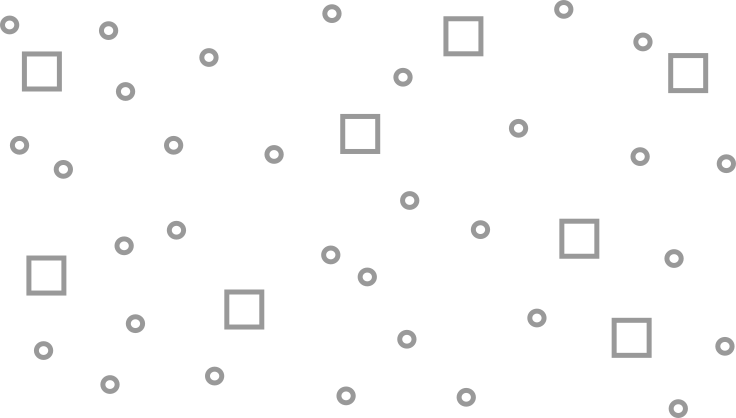
\includegraphics[width=\textwidth]{Factories-Customers.png}
		\caption{Factories represented by squares. customers represented by circles.}
	\end{subfigure}
	\hfil
	\begin{subfigure}[t]{0.4\textwidth}
		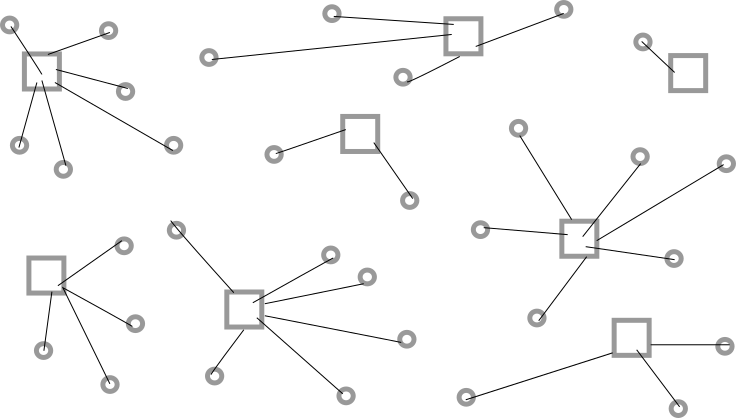
\includegraphics[width=\textwidth]{Factories-Customers-Assignation.png}
		\caption{Factories represented by squares. customers represented by circles. Assignation of a factory to a customer represented by a line.}
	\end{subfigure}	
\end{figure}

Gaspard Monge was a French mathematician who introduced for the very first time the optimal transport problem as \textit{d\'eblais et remblais} in 1781. Monge was interested in finding a map that distributes an amount of sand or soil extracted from the earth or a mine distributed according to a density $f$, onto a new construction whose density of mass is characterized by a density $g$, in such a way the average displacement is minimal. We see that Monge presented a more continuous flavor of the problem. \\

We remark that we are not interested in the quantity of mass we are transporting. This information it is not relevant for the problem or has no sense its consideration (for example the factories-customer problem). We are interested in finding a way to assign or distribute elements among two sets. We are interested in applications concerning the transportation of a finite amount of mass. Therefore, it is reasonable to state our problem in terms of probability measures.  \\

Formally, given two densities of mass $f$ and $g$, Monge was interested in finding a map $T:\Real^3\rightarrow\Real^3$ pushing the one onto the other,

\begin{equation*}
	\int_A g(y) \dy = \int_{T^{-1}(A)} f(x) \dx  \label{eq: Integral-Borel-MP}
\end{equation*}
For any Borel subset $A\subset\Real^3$. And the transport also should minimize the quantity, 
\begin{equation*}
	\int_{\Real^3} \abs{x-T(x)} f(x)\dx
\end{equation*}

Therefore, we need to search for the optimum in the set of measurables maps $T:X \rightarrow Y$ such that the condition \eqref{eq: Integral-Borel-MP} is translated to,

\begin{equation}
	(T_\#\mu)(A)=\mu(T^{-1}(A))\qquad \text{  for every measurable set } A\subset X.
\end{equation}
In other words, we need $T_\# \mu = \nu$.  Notice that given the context for which the problem was formulated, originally it was binded to $\Real^3$ or $\Real^2$ but we can consider the general case in $\Real^d$. In the Euclidean frameworks if we assume $f$, $g$ and $T$ regular enough and $T$ also injective, this equality implies,
\begin{equation}
	g(T(x))\det\parentheses{\D T(x)}=f(x) \label{eq: PDE Monge condition.}
\end{equation} 
\begin{figure}[H]
	\centering
	\caption{Monge problem. Finding a map.}
	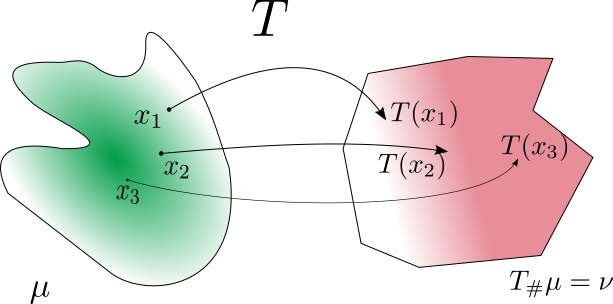
\includegraphics[width=0.4\textwidth]{Monge-Problem-densities.png}
\end{figure}

The equation \eqref{eq: PDE Monge condition.} is nonlinear in $T$ making difficult the analysis of the Monge's Problem. Moreover, the constrain makes this problem hard to handle since it is not close even under weak convergence. 


To appreciate this fact, consider $\mu = \Lebesgue^1\measurerestr[0,1]$ and the hat functions $h_k$ defined as follow,

\begin{equation*}
	h_k(x)=\begin{cases}
		2kx & x\in\brackets{0, \frac{1}{2k}}\\
		2-2kx & x\in \left(\frac{1}{2k}, \frac{1}{k}\right] \\
		0 & \otherwise
	\end{cases}
\end{equation*}
Then take the sequence $f_n:[0,1]\rightarrow [0,1]$,
\begin{equation}
	f_n(x)=\sum_{i=0}^{n-1}h_n\parentheses{x-\frac{i}{n}}
\end{equation}


We see that the sequence satisfies $\Tmeasure{\mu}{f_{n}}=\mu$. It is easy to check that $\mu\parentheses{f_n^{-1}\left(A\right)}=\Lebesgue^1\parentheses{A}$ for every open set $A\in [0,1]$. In the other hand, this is sequence of oscillating function converges weakly to its mean value $f_n\weakconvergence f=\frac{1}{2}$ by means of the Riemmann-Lebesgue theorem\footnote{Let $u\in L^p_{\mathrm{loc}}(\Real^N)$, be $Q-$ periodic, i.e. $u(x+e_i)=u(x)$ for any canonical basis $e_i$ of $\Real^N$, with $1\leq i\leq N$. For every $\epsilon>0$ and any $x\in\Real^N$, we set $u_\epsilon(x)=u(x/\epsilon)$. Then $u_\epsilon\weakconvergence \bar{u}$ in $L(E)$ for every bounded measurable set $E\subset \Real^N$ where $\bar{u}=const=\int_{Q(0,1)}u(y)\dy$. We can find the proof of this theorem in \cite{Fonseca2007ModCalculculusofVar} in the section of \emph{Weak convergence for $L^p$ spaces}.}, which makes $\Tmeasure{\mu}{f}\neq\Lebesgue^1\measurerestr [0,1]$.
\begin{figure}[H]
	\begin{center}
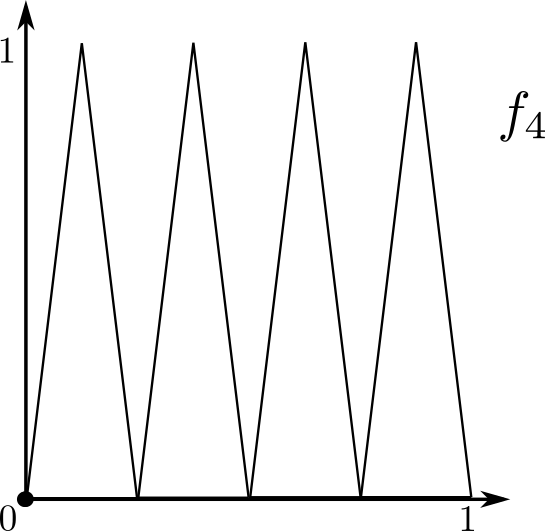
\includegraphics[width=0.5\textwidth]{OscillatingMeasure}
\caption{$f_n$ constructed using hat functions. The pictures shows the case $n=4$.}
	\end{center}
\end{figure}

\begin{problem} Given two probability measures $\mu \in \PlanSp\parentheses{X}$ and $\nu \in \PlanSp\parentheses{Y}$ and a cost function $c: X \times Y \rightarrow \braces{0, +\infty}$, the Monge's problem consists in finding a map $T:X\rightarrow Y$
	
\begin{equation}
\inf\braces{\Monge:=\int_X c(x, T(x)) \diff \mu(x): \quad \Tmeasure{\mu}{T}=\nu }\label{eq: Monge's Problem.}\tag{MP}
\end{equation}
\end{problem}

Monge analyzed geometric properties of the solution to this problem. Although, the question for the existence of an optimal map stayed open until a Russian mathematician named Leonid Vitaliyevich Kantorovich introduced in the paper \cite{Kantorovich1942} a suitable framework to study its optimality conditions and prove the existence of a minimizer. \\

When we formulate our factories-customer problem through finding an assignation map, we are excluding the situations in which one customer can be supplied by two or more factories, or in the case of the Monge's problem we are ignoring the possibility of splitting a unit of mass into small pieces that can be assigned simultaneously to different places. \\

The idea behind Kantorovich's formulation is to consider the transportation maps from one space to another as transportation plans, that is joint probability measures with their marginals given by the initial and final configurations.\\

Instead of assigning an element of $Y$ to each element of the set $X$, we can see the problem from a different perspective and assign a weight to the importance of the point $\left(x, y\right)\in X\times Y$. We would like to know how much of our total material is distributed from $x$ to $y$, in such a way to be consistent with information we have the initial and final material configuration. That is, we would like to know the optimal way to concentrate mass to the points $(x, y)$ in such a way we are not creating neither destroying mass. \\

Designing the transportation strategy using the above procedure is called a transport plan. In terms of probability theory, we are constructing a joint probability measure for $X\times Y$ with marginals given by the measures $\mu \in \PlanSp(X)$ and $\nu \in \PlanSp(Y)$. \\

Please note that in contrast to a map, we can always assign to a point $x\in Y$ as many points in $Y$ as we want, just considering the constraints given by the densities $\mu$ and $\nu$. We introduce the following notation to give the necessary formalism to this approach. 

\begin{definition}[Coupling]
Let $\mu$ and $\nu$ be probability measures over the measurable spaces $\parentheses{X, \mathcal{A}_X}$ and $\parentheses{Y, \mathcal{A}_Y}$. Finding a coupling between $\mu$ and $\nu$ means to construct a probability measure $\gamma$ on the space $X\times Y$ (precisely on the product $\sigma$-algebra $\mathcal{A}_X\otimes\mathcal{A}_Y$), $\mu$ and $\nu$ are admitted as marginals on $X$ and $Y$ respectively. That is $\gamma\geq 0$, $\gamma(X\times Y)=1$, $\Tmeasure{\gamma}{\proj_x}=\mu$ and $\Tmeasure{\gamma}{\proj_y}=\nu$. \label{def: Coupling}
\end{definition}
 

The above definition is equivalently to say that coupling two measures means to find a probability measure $\gamma$, such that for all measurable sets $A\subset X$ and $B\subset Y$, one has $\gamma\brackets{A\times Y}=\mu\brackets{A}$, $\gamma\brackets{A\times X}=\nu\brackets{B}$.

Moreover, for all integrable (nonnegative measurable) functions $\phi, \psi$ on $X$ and $Y$,
\begin{equation*}
	\int_{X\times Y}\parentheses{\phi(x)+\psi(y)}\diff\gamma(x,y)=\int_{X}\phi\dmu+\int_{Y}\psi\dnu
\end{equation*}

Since definition \ref{def: Coupling} is given for measures on probabilistic spaces, we can rephrase it in terms of stochastic variables. Let $(X, \mu)$ and $(Y, \nu)$ be two probability spaces. Coupling $\mu$ and $\nu$ means constructing two random variables $\X$ and $\Y$ on some probability space, such that $\law(\X)=\mu$, $\law(\Y)=\nu$. The couple $\parentheses{\X,\Y}$ is called a coupling of $\parentheses{\mu, \nu}$. \\


We use the notation $\Pi(\mu, \nu)$ to refer the \textbf{set of couplings} of $\mu$ and $\nu$. That is,

\begin{equation}
\Pi(\mu, \nu)=\braces{\gamma \in \PlanSp\parentheses{X\times Y}: \Tmeasure{\gamma}{\parentheses{\proj_x}}=\mu \ \mand \ \Tmeasure{\gamma}{\parentheses{\proj_x}}=\nu}
\end{equation}

\begin{lemma}[Existence of a coupling]
	\label{lm: Existence of a coupling}
Let $\mu$ and $\nu$ be probability measures over the measurable spaces $\parentheses{X, \mathcal{A}_X}$ and $\parentheses{Y, \mathcal{A}_Y}$. Then, there exists  $\exists \gamma \in \PlanSp(X\times Y)$, such that $\gamma\in\Pi(\mu, \nu)$.
\end{lemma}
\begin{proof}
	Take $\gamma=\mu\otimes\nu$.
\end{proof}


Notice that this approach to solve the problem is more general, since we can always create a transportation plan given a transportation map, i.e.

\begin{equation*}
\Tmeasure{\mu}{(\id, T)}=\gamma \in \PlanSp(X\times Y)
\end{equation*}

If $T$ is a transportation map it is easy to check that indeed $\Tmeasure{\gamma}{\parentheses{\proj_x}}=\mu$ and $\Tmeasure{\gamma}{\parentheses{\proj_y}}=\nu$.  This inspires a definition for a coupling between two measures generated by a transport map. \\


\begin{definition}[Deterministic Coupling]
Let $\parentheses{X, \mu}$ and $\parentheses{Y, \nu}$ be two probabilistic spaces. If there exists a measurable map $T:X\rightarrow Y$ such that $\Tmeasure{\mu}{T}=\nu$. We call the measure $\Tmeasure{\mu}{\parentheses{\id, T}}=\gamma \in \PlanSp(X\times Y)$ a deterministic coupling of $\mu$ and $\nu$.
\end{definition}

For the sake of simplicity, we refer as $\gamma_T$ a transportation plan generated from a transportation map $T$.


In terms of stochastic variables, a coupling $(\X,\Y)$ is said to be deterministic if there exists a measurable function $T: X \rightarrow Y$ such that $\Y = T(\X)$. Equivalently, $\parentheses{\X, \Y}$ is a deterministic coupling of $\mu$ and $\nu$, if its law $\gamma=\law(\parentheses{\X,\Y})$ is concentrated on the graph of a measurable map $T:X\rightarrow Y$. Other way to rephrase it is saying that $\mu=\law(\X)$, $\Y=T(\X)$, where $T$ is a change of variables from $\mu$ to $\nu$, for all $\nu$-integrable (nonnegative measurable)  function $\phi$,

\begin{equation*}
	\int_Y \phi(y)\dnu(y) = \int_X \phi(T(x))\dmu(x).
\end{equation*}

The increasing rearrangement on $\Real$ is an example of a coupling between two probability measures over one dimensional euclidean space. Let $\mu$, $\nu$ be two probability measures on $\Real$. Define their cumulative distribution functions by,
\begin{equation*}
	F(x)=\int_{-\infty}^{x}\dmu, \qquad G(y)=\int_{-\infty}^{y}\dnu	
\end{equation*}

Cumulative distributions not always are invertible, since they are not always strictly increasing. Although we can define their pseudo-inverses as follow,
\begin{align}
	F^{-1}(t)=\inf\braces{x\in \Real; F(x)>t}, \label{eq: Increasing rearregement F}\\
	G^{-1}(t)=\inf\braces{y\in \Real; G(y)>t}. \label{eq: Increasing rearregement G}
\end{align}
Then, we set the map $T$ as $T=G^{-1}\circ F$. If $\mu$ is atomless then $\Tmeasure{\mu}{T}=\nu$.

The increasing rearrangement coupling is useful to construct the \textit{Knothe-Rosenblatt coupling} between two Stochastic variables $\Real^n$. Let $\mu$ and $\nu$ be two probability measures on $\Real^n$, such that $\mu$ is absolutely continuous with respect to Lebesgue measure. This coupling is constructed in the following way:

\begin{enumerate}
	\item Take the marginal of the first projection on the first variable; this gives probability measures $\mu_1\parentheses{\dx_1}$, $\nu_1\parentheses{\dy_1}$ on $\Real$, with $\mu_1$ being atomless. Then define $y_1=T_1(x_1)$ by the composition of the pseudo-inverse functions of the increasing rearrangement, with $F$ and $G$ considered as they are in \eqref{eq: Increasing rearregement F} and \eqref{eq: Increasing rearregement G} respectively.
	
	\item Now take the marginal on the first two variables and disintegrate it with respect to the first variable. This gives probability measures $\mu_2\parentheses{\dx_1\dx_2}=\mu_1(\dx_1)\mu_2\parentheses{\dx_2 |x_1}$, $\nu_2 (\dy_1\dy_2)=\nu_1(\dy_1)\nu_2\parentheses{\dy_2|y_1}$. For each given $y_1\in \Real$, we set $y_1=T_1(x_1)$, and then we define $y_2=T_2(x_2; x_1)$ under the increasing rearrangement formula of $\mu\parentheses{\dx_2| x_1}$ into $\nu\parentheses{\dy_2| y_1}$.
	
	\item We repeat the construction, adding one variable after another. For example, after the assignation $x_1\rightarrow y_1$ has been determined, the conditional probability of $x_2$ is seen as a one-dimensional probability on a small slice of width $\dx_1$, and it can be transported to the conditional probability of $y_2$ seen as one dimensional probability of a slice of width $\dy_1$. After $n$ constructions, this procedure maps $\Y=T(\X)$.
\end{enumerate} 

The \textit{Knothe-Rosenblatt coupling} has the property that its Jacobian matrix for the change of variable $T$ is upper triangular with positive entries on the diagonal. 	


\begin{lemma}[Gluing lemma] If $\Z$ is a function of $\Y$ and $\Y$ is a function of $\X$, then $\Z$ is a function of $\X$. Let $(X_i , \mu_i)$, $i = 1, 2, 3$,  be Polish probability spaces. If $(\X_1 , \X_2)$ is a coupling of $(\mu_1, \mu_2 )$ and $(\Y_2 , \Y_3)$ is a coupling of $(\mu_2, \mu_3)$, then it is possible to construct a triple of random variables $(\Z_1 , \Z_2, \Z_3)$ such that $(\Z_1, \Z_2)$ has the same law as $(\X_1 ,\X_2)$ and $(\Z_2, \Z_3)$ has the same law as $(\Y_2, \Y_3)$.
\end{lemma}


\begin{problem}Given $\mu \in \PlanSp\parentheses{X}$, $\nu \in \PlanSp\parentheses{Y}$, and $c: X\times Y \rightarrow \brackets{0, +\infty}$, we consider the problem
	\begin{equation}
		\Theta(\mu, \nu)=\inf\braces{\Kantorovich := \int_{X\times Y} c \diff\gamma : \qquad \gamma \in \TransPlansSet{\mu}{\nu}}\label{eq: Kantorovich's Problem.}\tag{KP}
	\end{equation}
where $\TransPlansSet{\mu}{\nu}$ is the set of \textit{transport plans}.
\end{problem}

It is a fact for The Kantorovich's formulation that it is always possible to find a transport plan, to see this fact it is enough to take $\gamma=\mu\otimes \nu$, as shown in lemma \ref{lm: Existence of a coupling}. By contrast, it is not always possible to find transportation maps (deterministic couplings).\\

Consider a measure $\mu$ on $\Real^d$, concentrated on $N$ different atoms $x_i \in \Real^d$, 
\begin{equation*}
\mu=\frac{1}{N}\sum_{i=0}^{N-1} \delta_{x_i}
\end{equation*} 

Where $\delta_{x_i}$ is the Dirac mass at point $x_i$. Consider $N$ open balls on $\Real^d$ centered at $x_i$ with radius $\epsilon_i > 0$, such that they disjoint pairwise. Let $D=\bigcup_{i=0}^{N-1} \ball{x_i}{\epsilon_i}$ be the union of these balls. Let $\nu$ be a the Hausdorff measure of over $D\subset \Real^d$. That is $\nu=\Hausdorff\measurerestr D$. We see that it is impossible to couple $\mu$ and $\nu$ deterministically; since there is no map $T$, such that $\Tmeasure{\mu}{T}=\nu$. \\

\begin{figure}[H]	
	\begin{center}
	\caption{Transportation maps. There is no deterministic coupling for $\mu$ and $\nu$, but there is a transportation plan.}
	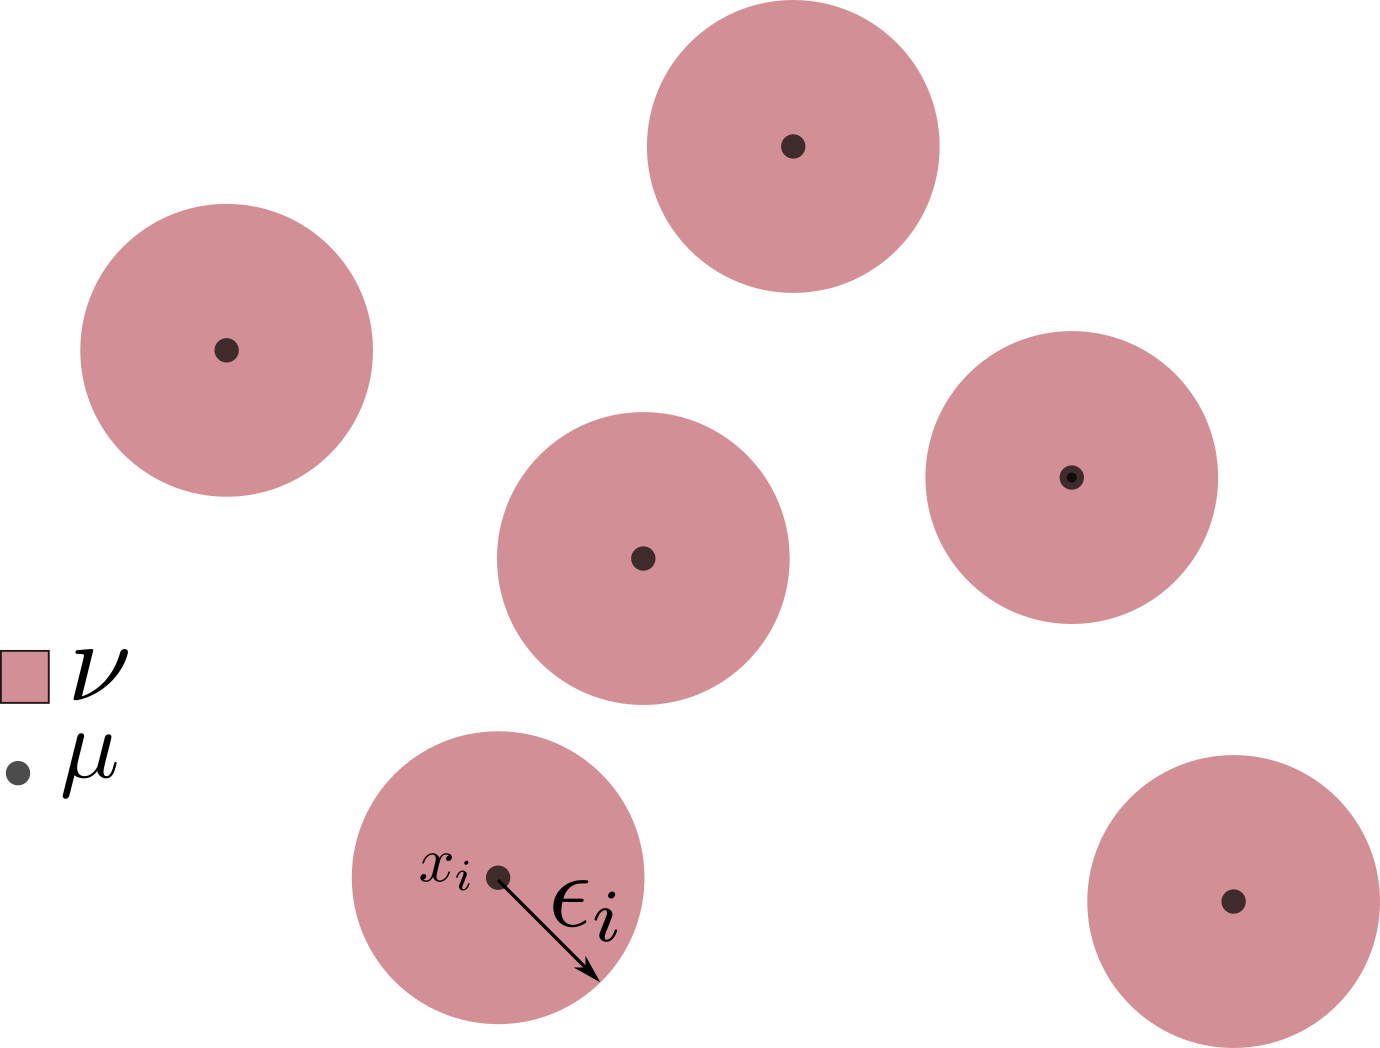
\includegraphics[width=0.5\textwidth]{No-Transport-Map.png}
	\label{fig: No deterministic coupling.}
	\end{center}	
\end{figure}



\subsection{Existence of a minimizer for Kantorovich's Problem.}


\subsubsection{Properties of transportation plans.}
\begin{lemma}
	Let $X$ be a metric space. If $f:X\rightarrow\Realex$ is a lower semi-continuous function, bounded from below, then the functional  $J:\PMeasureSp(X)\rightarrow \Realex$ defined on the space of finite positive measures on $X$, given by
	\begin{equation*}
	J(\mu)=\int f \dmu
	\end{equation*} 
	is lower semi-continuous for the weak convergence of measures. \label{lemma: Monotone Convergence implies l.s.c}
\end{lemma}
\begin{proof}
	Let $(f_n)_{n\in \Naturals}$ be a sequence of continuous and bounded functions, converging increasingly to $f$. Consider the functionals $J_n: \PMeasureSp(X)\rightarrow\Realex$, defined as
	\begin{equation*}
	J_n(\mu)=\int f_n \dmu
	\end{equation*}	
	Every $J_n$ is continuous for the weak convergence. We set $J(\mu)=\int f \dmu$. We see that $J_n(\mu) \leq J(\mu)$ for any $\mu$. Since our functions are bounded, and $f$ is bounded from below, and our measures are finite, we can make use of monotone convergence theorem, $J_n(\mu)\rightarrow J(\mu)$, having as result $J(\mu)=\sup_{n} J_n(\mu)$. Since we have that $J(\mu)$ is the supremum of continuous functions we can assure that that $J$ is lower semicontinuous.
\end{proof}
\begin{theorem}[Lower-semicontinuity of the cost function]
	Let $X$ and $Y$ two Polish spaces, and $c:X\times Y\rightarrow\Real\cup\braces{+\infty}$ is a real valued lower semicontinuous function bounded from below. Then the functional $K:\PlanSp(X\times Y)\rightarrow \Real\cup\braces{+\infty}$, 
	\begin{equation}
	K(\gamma):=\int_{X\times Y}c\diff\gamma,
	\end{equation}
	is lower semicontinuous. \label{th: l.s.c of c.}
	\begin{proof}
		This is a consequence of lemma \ref{lemma: Monotone Convergence implies l.s.c} setting $f=c$ over $X\times Y$.
	\end{proof}

The beauty of Kantorovich's formulation lies on the fact that the set of transport plans is compact under weak convergence making it a suitable framework where we can use the Weierstrass' criterion to show the existence of a minimizer. 

\begin{theorem} Let $X$ and $Y$ be compact metric spaces, $\mu \in \PlanSp(X)$, $\nu \in \PlanSp(Y)$ and a cost function $c: X\times Y \rightarrow \Real$ a continuous function. Then \eqref{eq: Kantorovich's Problem.} admits a solution.
\end{theorem}
\begin{proof}
	To prove the existence we make use of the Weierstrass’ criterion for existence of minimizers. Therefore, we need to prove that $\Kantorovich$ is at least lower semicontinuous and compactness of the space $\Pi(\mu, \nu)$ under some topology. 
	
	We choose as a notion of convergence the weak convergence of probability measures in duality with $C_b(X\times Y)$. This immediately implies continuity for $\Kantorovich$ by definition since $c$ is already in $C(X\times Y)$ defined in a compact space $X\times Y$. 
	
	Now take a sequence $\parentheses{\gamma_n}_{n\in\Naturals} \in \Pi(\mu, \nu)$. Since they are probability measures for all $n$ they are bounded in the dual of $C(X\times Y)$.  weak-* compactness in the dual of compact metric spaces guarantees the existence of a convergent subsequence $\gamma_{n_k} \weakconvergence \gamma$. Let us fix $\phi \in C(X)$ and using $\int\phi(x) \diff \gamma_{n_k}=\int \phi \dmu$ and taking the limit we have $\int_{X\times Y}\phi(x) \diff \gamma=\int_{X} \phi \dmu$. In this way we prove that $\Tmeasure{\parentheses{\proj_x}}{\gamma}=\mu$.  We can repeat this argument for $\nu$, fixing $\psi \in C(Y)$ and taking the limit of $\int_{X\times Y} \psi(y) \diff \gamma_{n_k}=\int \psi \dnu$, implies $\int_{X\times Y} \psi(y) \diff \gamma=\int \psi \dnu$. 
	
	This proves that $\Tmeasure{\parentheses{\proj_y}}{\gamma}=\nu$. Hence, the limit $\gamma \in \Pi(\mu, \nu)$ showing that the set of couplings of $\mu$ and $\nu$ is sequentially compact. 
\end{proof}

Continuity for the cost function and compactness of the metric spaces can be demanding requirements. However we can substitute them by milder conditions for the existence of a minimizer. 

\begin{theorem}
	Let $X$ and $Y$ be compact metric spaces, $\mu \in \PlanSp(X)$, $\nu \in\PlanSp(Y)$, and $c:X\times Y\rightarrow \Realex $  be lower semi-continuous and bounded from below. Then Kantorovich's problem admits a solution.
\end{theorem}

\begin{proof}
By theorem \ref{th: l.s.c of c.}, the functional $K(\gamma) =\int c\diff\gamma$ is lower semicontinuous. We apply again Weierstrass criterion proving existence of a minimizer.
\end{proof}


\begin{lemma}
	The set of couplings $\Pi(\mu, \nu)$ between two probability measures $\mu$ and $\nu$ defined over two Polish spaces $X$ and $Y$ respectively, is tight.
\end{lemma}
\begin{proof}
Fix $\epsilon>0$ and find two compact sets $K_x\subset X$ and $K_y\subset Y$ such that $\mu\parentheses{X\backslash K_x}<\epsilon$, and $\nu\parentheses{Y\backslash K_y}<\epsilon$. Then the set $K_X\times K_Y$ is compact in $X\times Y$ and, for any $\gamma_n\in \Pi(\mu, \nu)$, we have,
\begin{align*}
\gamma_n\parentheses{(X\times Y)\backslash \parentheses{K_X\times K_Y}}&\leq \gamma_n\parentheses{(X\backslash K_X)\times Y}+\gamma_n\parentheses{X\times \parentheses{Y\backslash K_y}}\\&=\mu\parentheses{X\backslash K_X}+\nu\parentheses{Y\backslash K_Y}\\&=2\epsilon
\end{align*}  
Given the arbitrary way to choose $\epsilon$, $\Pi(\mu,\nu)$ is tight.
\end{proof}
\begin{theorem}
Let $X$ and $Y$ be Polish spaces, and $c:X\times Y \rightarrow \Realex_+$, a real valued lower semi-continuous cost function on the space $X\times Y$. Then the Kantorovich's problem \eqref{eq: Kantorovich's Problem.} admits a solution.
\end{theorem}

\begin{proof}
 By Prokhorov the tightness of transport plans, we have relatively compactness of the transport plans and lower semicontinuity of the cost function. Applying Weirestrass criterion we obtain the existence of an optimizer.
\end{proof}


\subsection{Properties of Optimal plans}
\begin{theorem}[Convexity of optimal plans]
	The set of solutions $\bar\gamma\in\Pi(\mu,\nu)$ for the Kantorovich's problem is a convex set.
\end{theorem}
\begin{proof}
	We see immediately that if $\gamma_1$ and $\gamma_2$ solve the Kantorovich's problem, for any $t\in[0,1]$, the plan $\gamma=t\gamma_1+(1-t)\gamma_2$, also solves the problem. 
\end{proof}
\end{theorem}
An interesting property of an optimal coupling between two measures, is that optimality remains after restricting the plan to a non zero measure subset of $X\times Y$. 
\begin{theorem}[Optimality is inherited by restriction]
	Let $(X, \mu)$ and $(Y, \nu)$ be two Polish spaces, $a \in L^1(\mu)$, $b \in L^1(\nu)$, let $c : X \times Y \rightarrow
	\Real\cup \braces{+\infty}$ be a measurable cost function such that $c(x, y) \geq a(x) + b(y)$ for all x, y; and let $\Theta(\mu, \nu)$ be the optimal transport cost from $\mu$ to $\nu$.
	Assume that $\Theta(\mu, \nu)<\infty$  and let $\gamma \in \Pi(\mu,\nu)$ be an optimal transport plan. Let $\tilde\gamma$ be a nonnegative measure on $X\times Y$, such that $\tilde \gamma\leq \gamma$ and $\tilde \gamma(X\times Y)>0$. Then the joint probability measure,
	\begin{equation*}
	\hat\gamma = \frac{\tilde\gamma}{\tilde\gamma(X\times Y)}
	\end{equation*}
	is an optimal plan between its marginals $\hat\mu=\Tmeasure{\hat \gamma}{(\proj_X)}$ and $\hat\nu =\Tmeasure{\hat \gamma}{(\proj_Y)}$. 	
\end{theorem}

\begin{proof}
	We proceed by contradiction; take a transportation plan $\hat \gamma$ such that  for a given cost function $c$, it is not optimal. Since $\hat \gamma$ is not optimal we can find another plan $\overline \gamma$ such that $\Tmeasure{\overline \gamma}{(\proj_X)}=\Tmeasure{\hat \gamma}{(\proj_X)}=\hat \mu$ and $\Tmeasure{\overline \gamma}{(\proj_Y)}=\Tmeasure{\hat \gamma}{(\proj_Y)}=\hat \nu$ and $K(\overline\gamma)<K(\hat \gamma)$.
	
	Let $\alpha=\tilde\gamma(X\times Y)>0$ be the measure of the space under $\tilde{\gamma}$ which is greater than zero by definition. Let $\gamma' = (\gamma-\tilde\gamma) + \alpha\overline{\gamma}$ be a measure over $X\times Y$. We see that 
	$\gamma'>0$ by construction since $\gamma$
	
	\begin{align*}
	\gamma' =& (\gamma-\tilde\gamma) + \alpha\overline{\gamma} \\
	=&\gamma-\frac{\tilde{\gamma}(X\times Y)}{\tilde{\gamma}(X\times Y)}\tilde\gamma + \alpha\overline{\gamma} \\
	=& \gamma-\tilde{\gamma}(X\times Y)\hat{\gamma} +\tilde\gamma(X\times Y)\overline{\gamma} \\
	=&\gamma+\alpha\parentheses{\overline{\gamma}-\hat{\gamma}}\\
	<&\gamma
	\end{align*}
	
	$\overline \gamma$ and $\tilde \gamma$ share the same marginals, therefore $\Tmeasure{\gamma'}{(\proj_X)}=\Tmeasure{\gamma}{(\proj_X)}$ and 
	$\Tmeasure{\gamma'}{(\proj_Y)}=\Tmeasure{\gamma}{(\proj_Y)}$ giving as result that $\gamma' \in \Pi(\mu, \nu)$, contradicting the fact that $\gamma$ is optimal.
\end{proof}
The last theorem tells us that transferring part of the initial mass to part of the final using the optimal plan designed for the total mass is also optimal. 
\begin{corollary}
	Under the framework of the last theorem, if $\gamma$ is the unique optimal transference plan between $\mu$ and $\nu$, then also $\hat\gamma$ is the unique optimal transference plan between $\hat\mu$ and $\hat\nu$.
\end{corollary}

\begin{proof}
	Let $\gamma$ be the unique optimal coupling between $\mu$ and $\nu$. Let $\overline\gamma$ be any optimal transfer plan coupling $\hat{\mu}$ and $\hat{\nu}$. Define $\gamma'$ as we did in the last proof $\gamma'=(\gamma-\tilde{\gamma})+\alpha\overline{\gamma}$, with $\alpha=\tilde\gamma(X\times Y)$. This implies that $K(\gamma')=K(\gamma)$. Since the coupling for $\mu$ and $\nu$ is unique $\gamma'=\gamma$, which implies $\tilde\gamma=\alpha\gamma$ then $\tilde{\gamma}=\hat{\gamma}$ 
\end{proof}

\section{Kantorovich's formulation as relaxation of Monge's formulation.}

There are situations in which is possible to find a deterministic coupling between two measures, but not an optimal one for a cost function $c:X\times Y \rightarrow \Realex$. A common example, popular in the literature, is the following: consider as cost function $c:\Real^2\times\Real^2 \rightarrow \Real$, the Euclidean distance $c(x,y)=\abs{x-y}$, the measure $\mu=\Hausdorff\measurerestr D$ as the Hausdorff measure for the segment  $D=\braces{\parentheses{0, t}^\top \in \Real^2:\, \text{ for } t\in [0,1]}$. 

Let $D_1$ and $D_2$ be the segments given by,
\begin{align*}
D_1 = \braces{\parentheses{-1, t}^\top\in\Real^2:\, \text{ for } t\in [0,1]} \\
D_2 = \braces{\parentheses{+1, t}^\top\in\Real^2:\, \text{ for } t\in [0,1]}
\end{align*}

And we set the measure $\nu$ as follows, 
\begin{equation*}
\nu=\frac{\Hausdorff\measurerestr D_1 + \Hausdorff \measurerestr D_2}{2}
\end{equation*}

\begin{figure}[H]
	\begin{center}
	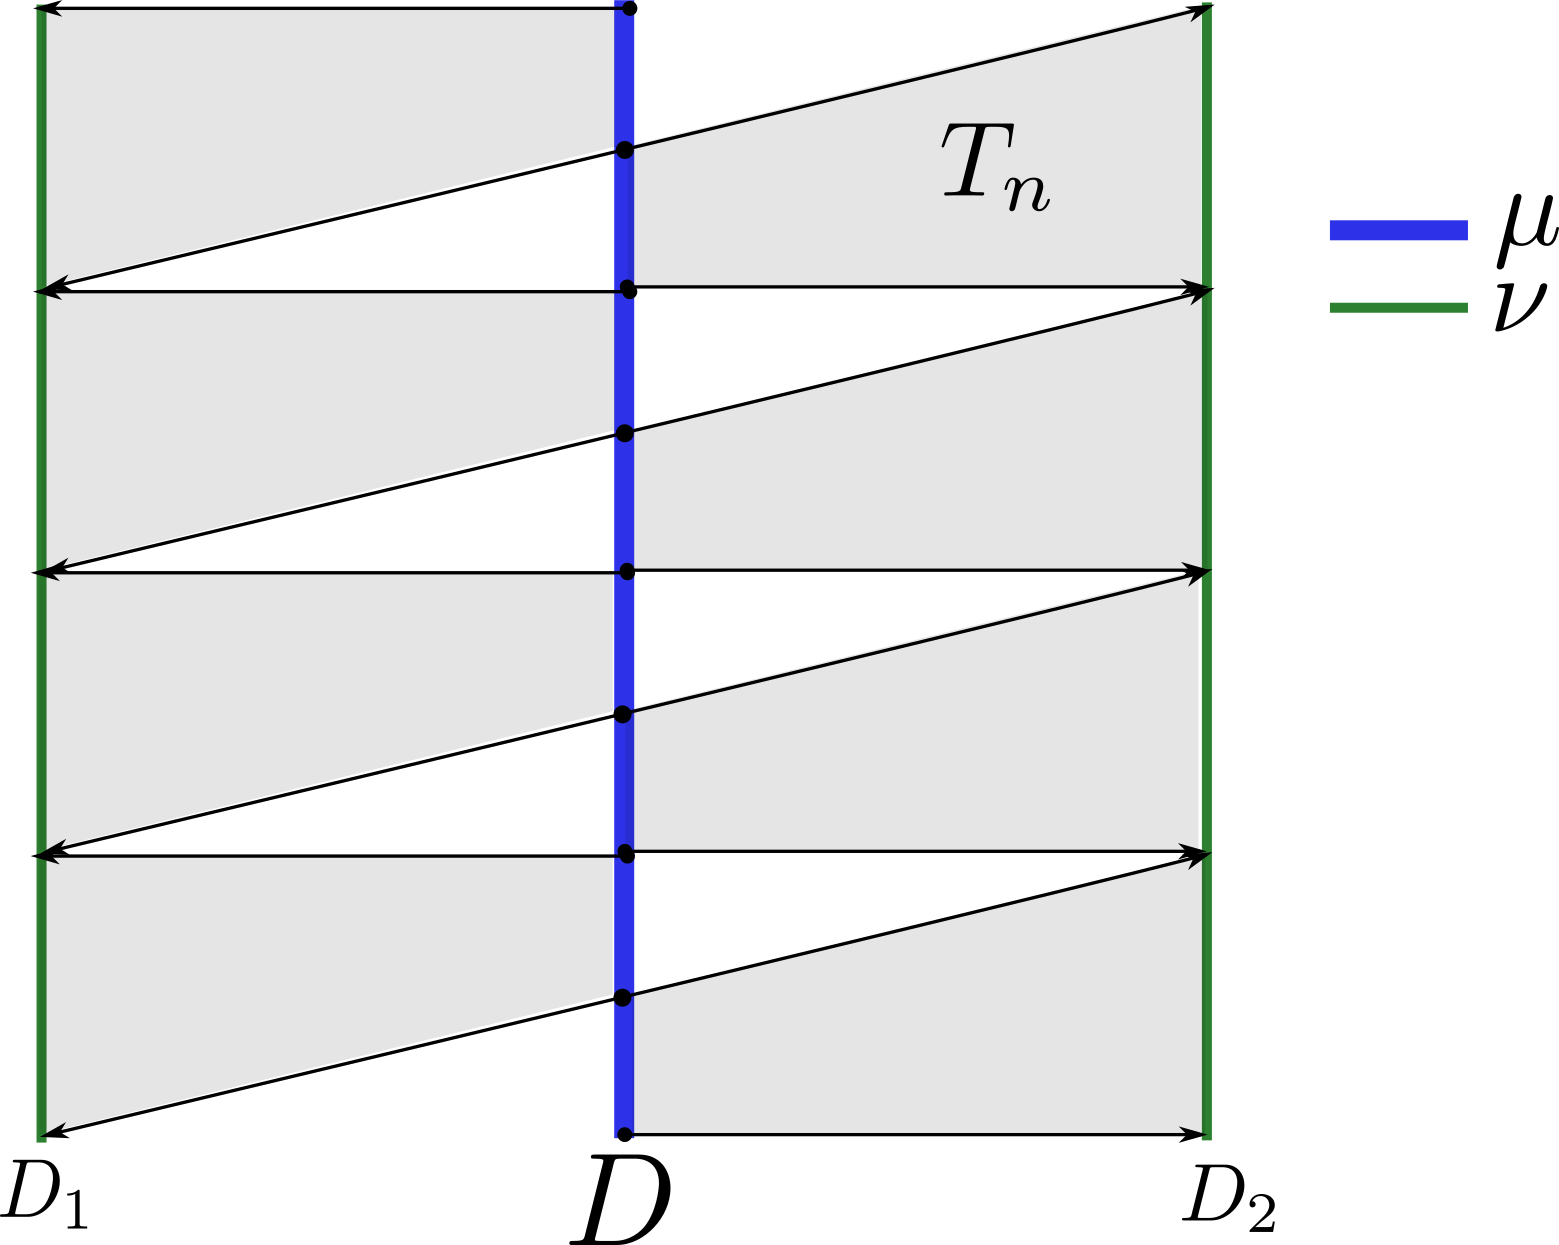
\includegraphics[width=0.5\textwidth]{No-Optimal-Transport.png}
	\caption{There is a deterministic coupling for $\mu$ and $\nu$, but no optimal one. The map $T_n$ shown in this picture with $n=4$.}	
	\end{center}

\end{figure}


There are many ways to construct a transportation map for this situation. Consider the maps $T_n$ constructed splitting the segment $D$ into $2n$ equal parts and the segments $D_1$ and $D_2$ in $n$ equal parts. We label the parts of the segment $D$ with the integer numbers from $0$ to $2n-1$. Then the map $T_n$ assign the parts of $D$ labeled with even numbers to the right hand side segment $D_2$ and the parts labeled with odd numbers to the left right side segment $D_1$. 

Formally, let $k=0, \dots, 2n-1$ be an integer used to label the equal parts of $D$,

\begin{equation*}
T_n\parentheses{\begin{pmatrix}0\\t\end{pmatrix}\in D}=\begin{cases}
\begin{pmatrix}1\\  2t - \frac{k}{2n}\end{pmatrix} & k \text{ even } \mand \ t \in \left[\frac{k}{2n}, \frac{k+1}{2n}\right),  \\
\begin{pmatrix}-1 \\  2t- \frac{k+1}{2n}\end{pmatrix} &  k \text{ odd } \mand \ t \in \left(\frac{k}{2n}, \frac{k+1}{2n}\right].
\end{cases}
\end{equation*}

We can find an upper boundary for the total cost $C(T_n)$,

\begin{align*}
M(T_n)&=\int_{D}\abs{x-T_n(x)} \dmu(x)\\&=2n\int_{0}^{\frac{1}{2n}}\sqrt{1+4t^2} \dt\\ &\leq 2n\parentheses{\int_{0}^{\frac{1}{2n}}1+4t^2\dt}^{1/2}\parentheses{\int_{0}^{\frac{1}{2n}}\dt}^{1/2}\\ &= \sqrt{1+\frac{1}{3n^3}}\\&\leq 1+\frac{1}{n}
\end{align*}

Let $\gamma_{T_n}$ be deterministic coupling generated by $T_n$. We see that we can find always find a cheaper plan $\gamma_{T_{n+1}}$ for any $n\in \Naturals$. This sequence of transportation plans converges weakly to the plan $\gamma_{T_n}\weakconvergence \gamma_{T}=\frac{\gamma_{T^+}}{2}	+ \frac{\gamma_{T^-}}{2}$. Where $T^{+}$ and $T^{-}$ are given by:

\begin{align*}
T^{+}(x)&=x+\begin{pmatrix} 1 \\ 0\end{pmatrix}\\
T^{-}(x)&=x-\begin{pmatrix} 1 \\ 0\end{pmatrix}
\end{align*} 


The idea is that the mass of each point $x\in D$ is split in two and equally distributed among $D_1$ and $D_2$ assigning one half of the mass respectively. Note that this distribution is an optimal plan for the cost function $c(x,y)=\abs{x-y}$. Because of the triangle inequality, sending the mass from $x\in D$ to any other point of $D_1$ and $D_2$ different than those assigned by the maps $T^{\pm}$, implies a higher cost.


From the last example we see that a sequence of deterministic couplings converges to a transportation plan that is a solution for Kantorovich's problem \eqref{eq: Kantorovich's Problem.}, but clearly it is not for Monge's problem \eqref{eq: Monge's Problem.}. We also gave one example where \eqref{eq: Monge's Problem.} has no solution. Assume for a moment that Monge's  situation where indeed does exist a solution for Monge's problem, then the following question arises: Is there any situation where Monge's problem and Kantorovich's problem have the same solution?

\begin{lemma}
On a compact subset  ̋$\Omega \subset \Real^d$, the set of plans $\gamma_T$ induced by a transport is dense in the set of plans $\Pi(\mu, \nu) $ whenever $\mu$ is atomless.\label{lem: Density of maps.}
\end{lemma}

\begin{theorem}
On a compact subset $\Omega \subset \Real^d$,  $\Kantorovich$ is the relaxation of $J(\gamma)$. In particular, $\inf J = \min K$, and hence Monge and Kantorovich problems have the same infimum.
\end{theorem}
\begin{proof}
Since $K$ is continuous, then it is lower semicontinuous, and since we have $K\leq J$, then $K$ is necessarily smaller than the relaxation of $J$. We only need to prove that, for each $\gamma$, we can find a sequence of transports $T_n$ such that $\gamma_{T_n}\rightarrow \gamma$ and $J\parentheses{\gamma_{T_n}}\rightarrow K(\gamma)$, so that the infimum in the sequential characterization of the relaxed functional will be smaller than $K$, thus providing the equality. 

Actually, since for $\gamma=\gamma_{T_n}$ be two functionals $K$ and $J$ coincide, and since $K$ is continuous we only need to produce a sequence $T_n$ such that $\gamma_{T_n}\weakconvergence\gamma$. It is possible to do the last step due to the density of transport plans generated by a map $\gamma_{T_n}$ in the set of transport plans $\Pi(\mu, \nu)$.
\end{proof}

To understand the relation between both formulations we come back to the factories-customers example. The consortium instead of having the policy of assigning a factory to each costumer, they prefer a relaxation of the problem. Now, they consider their products as mass distributed across the city in different places given by the production rate of each factory that they need to redistribute to a given configuration, that is the costumers location with their respective demand. 

Approaching the problem in this way gives us the flexibility to supply each customer's demand with the production of many factories.  

\section{Cyclical Monotonicity and Duality.}

Imagine that the consortium changed its policy and it has decided not to be responsible any longer for the transportation of the goods, letting the customers to solve this problem by themselves (assume that the consortium has the monopoly of the goods and the customers have no choice but to adhere to this policy). An entrepreneur feeling that he can ship the goods more efficiently that the consortium did, he intend to buy the goods at the factories and selling them at the customers' stores. Then, he must negotiate with the consortium the prices $-\phi(x)$ that he is able to pay at each factory for the goods and the selling prices $\psi(y)$ at each customers' store. In order to succeed, he need to be competitive and should do it better than the consortium did. Therefore, he must be able that cover with the difference of the sale prices the transportation costs and they should be less than the consortium's costs $\psi(y)+\phi(x)\leq c(x,y)$. He is subject to this constraint and he should negotiate with the consortium and the customers the prices $\phi(x)$ and $\psi(y)$ in order to obtain the maximum profit.


\subsection{Duality}
We see that for any $\gamma \in \MeasureSp_+(X\times Y)$ we have,
\begin{equation}
\sup_{\phi, \psi} \parentheses{\int_X \phi\dmu +\int_Y\psi\dnu-\int_{X\times Y}\parentheses{\phi(x)+\psi(y)}\diff \gamma} = \indicator{\Pi(\mu,\nu)}{(\gamma)}=\begin{cases}
0 & \text{if } \gamma \in \Pi(\mu, \nu) \\
+\infty & \text{otherwise}.	
\end{cases}\label{eq: Constrain indicator}
\end{equation}
where the supremum is taken among all bounded and continuous functions $\phi$, $\psi$. 

Note that the result of this problem is $0$ if $\gamma$ satisfies the constrain of being a probability measure over $X\times Y$ with given marginals $\mu$ and $\nu$, and we obtain $\infty$ if $\gamma$ does not satisfy this constrain.

Therefore, we can rewrite the Kantorovich's transport problem as an unconstrained minimization problem,    
\begin{align}
	\Kantorovich&=\min_{\gamma}\parentheses{\int_{X\times Y} c\diff\gamma +\int_{X} \phi \dmu +\int_{Y} \psi\dnu - \int_{X\times Y}\parentheses{\phi(x)+\psi(y)}\diff\gamma} \\
	&=\sup_{\phi,\psi}\parentheses{ \int_{X}\phi\dmu+\int_{Y}\psi\dnu}+\min\parentheses{\int_{X\times Y}c(x,y)\diff\gamma-\sup_{\phi, \psi}\parentheses{\int_{X}\phi(x)\dmu+\int_{Y}\psi(y)\dnu}} \label{eq: Unconstrained Kantorovich with Perturbation.}
\end{align}
Note that,
\begin{equation}
\inf_{\gamma}\int_{X\times Y}\parentheses{c(x,y)-\parentheses{\phi(x)+\psi(y)}} \diff \gamma =\begin{cases}
	0 & \text{ if } \phi(x)+\psi(y)\leq c(x,y),\quad \forall (x,y)\in X\times Y \\
	-\infty & \text{otherwise}.
 \end{cases}
\end{equation}
In the other hand, equation \eqref{eq: Unconstrained Kantorovich with Perturbation.} it is not really useful if we are not able to exchange the $\min$ and $\sup$; for a moment suppose that the conditions that allow to exchange them do exist, we can rewrite the equation \eqref{eq: Unconstrained Kantorovich with Perturbation.} as follows,
\begin{equation}
	\Kantorovich=\sup_{\phi, \psi}\parentheses{\int_{X}\phi\dmu+\int_{Y}\psi\dnu+\inf_{\gamma}\int_{X\times Y}\parentheses{c(x,y)-\parentheses{\phi(x)+\psi(y)}}\diff\gamma}
\end{equation}

If it exists $(x,y) \in X\times Y$ such that $\phi(x)+\psi(y)>c$, we can find measures $\gamma$ concentrated on the set where the strict inequality holds and mass tending to infinity, sending the value of the integral to $-\infty$. The above equation motivates the dual formulation of the problem,

\begin{problem}
Given $\mu\in\PlanSp(X)$, $\nu\in\PlanSp(Y)$, and the cost function $c:X\times Y\rightarrow \Real_+$ we refer as the dual formulation of the transport problem \eqref{eq: Transportation Dual problem},
\begin{equation}
\Delta=\sup\braces{\int_X\phi\dmu+\int_Y\psi \dnu: \phi \in C_b(X),\ \psi \in C_b(Y),\ \phi(x)+\psi(y)\leq c(x,y),\ \forall (x,y)\in X\times Y} \tag{DP} \label{eq: Transportation Dual problem}
\end{equation}	
\end{problem}
Notice that for any $\gamma\in \Pi(\mu, \nu)$,
\begin{equation}
	\int_{X}\phi\dmu+\int_{Y}\psi\dnu=\int_{X\times Y} \phi(x)+\psi(y)\diff \gamma \leq \int_{X\times Y} c(x,y)\diff \gamma
\end{equation}

Then we see that the objective value of the dual problem is less or equal than the primal Kantorovich's problem, as long as the pair $(\phi, \psi)$ is admissible.


 Since the set of admissible maps is not compact we cannot assure the existence of a maximizer. To find the conditions needed to assure existence of the minimizer or a duality equality we need to characterize functions by means of $c-$concavity.

\begin{definition}
	Let $X$, $Y$ be two sets, let $c:X\times Y \rightarrow \Real$, a real valued cost function bounded from below. Given a function $\zeta: X\rightarrow \Real\cup\braces{-\infty}$, we define its $c$-concave transform of $\zeta$, the function $\zeta^c: Y\rightarrow \Realex$ by
	\begin{equation}
	\zeta^c(y)=\inf_{x\in X}\parentheses{c(x,y)-\zeta(x)}
	\end{equation}
	In similar way, we can define the $\bar{c}-$transform of $\xi: Y\rightarrow \Real\cup\braces{-\infty}$ by
	\begin{equation}
	\xi^{\bar{c}}(x)=\inf_{y\in Y}\parentheses{c(x, y)-\xi(y)}
	\end{equation}
	A function $\psi$ defined on $Y$ is said to be $\bar c-$concave if it is not identically to $-\infty$ and there exists $\zeta$ defined on $X$, such that $\psi=\zeta^c$. Similarly, a function $\phi$ defined on $X$ is said to be $ c-$concave if it is not identically to $-\infty$ and there exists $\xi$ defined on $Y$ such that $\phi=\xi^{\bar{c}}$.
\end{definition}

We use a bar to denote the difference between the transformation respect to the first and the second parameter of the cost function. This notation becomes trivial if we deal with symmetric cost functions.
For a given cost function $c:X\times Y\rightarrow \Real$. We denote by $c-conc(X)$ the set of $c-$concave  functions defined on $X$. In similar way, we denote by $\bar{c}-conc(Y)$ the set of $\bar{c}-$concave functions defined on $Y$. 

The following theorem encompass the importance of using $c$-characterization for functions, it represents a generalization for the convex envelop theorem.
\begin{theorem}\label{th: C-concave envelope}
Suppose that $c$ is real valued. For any $\phi: X\rightarrow \Real\cup \braces{-\infty}$, we have $\phi^{c\bar c}\geq \phi$. We have the equality $\phi^{c\bar c}=\phi$ if and only if $\phi$ is $c-$concave. Moreover, $\phi^{c\bar c}$ is the smallest $c-$concave function larger than $\phi$.
\end{theorem}
\begin{proof}
	Let $\phi^{c\bar {c}}$ be the $c$-transform of the $\bar{c}$-transform of $\phi$,
	\begin{align*}
		\phi^{c\bar c}(x)&=\inf_{y\in Y} \parentheses{c(x,y)-\phi^{c}(y)}\\
		&=\inf_{y\in Y} \parentheses{c(x,y)-\inf_{\tilde x\in X}\parentheses{c(\tilde x,y)-\phi(\tilde x)}}.
	\end{align*}
	
	Note that $\forall (x, y) \in X\times Y$,
	\begin{equation*}
		\inf_{\tilde x \in X}\parentheses{ c(\tilde x,y)-\phi(\tilde x) }\leq c(x, y) - \phi (x).
	\end{equation*}
	
	Therefore, 
	\begin{equation*}
		\phi^{c\bar c}(x)\geq \inf_{y\in Y}\parentheses{c(x,y)-c(x,y)+\phi(x)}=\phi(x)
	\end{equation*}
	As we did for $\phi$, we can repeat the above arguments for any $\xi:Y\rightarrow \Real\cup\braces{-\infty}$, having as result $\xi^{\bar{c}c}\geq\xi$. 
	If $\phi$ is $c-$concave, there exists $\xi$ allowing to write $\phi$ as $\phi=\xi^{\bar{c}}$.  Therefore, using the fact that $\xi^{\bar{c}c}\leq \xi$, 
	\begin{align*}
		\phi^{c\bar c}(x)&=\inf_{y\in Y} \parentheses{c(x,y)-\phi^c(y)}\\
						&\leq \inf_{y\in Y}\parentheses{c(x,y)-\xi}
						\\
						&=\xi^{\bar{c}}=\phi
	\end{align*}
	Proving in this way that if $\phi \in c-conc(X)$, then $\phi^{c\bar c}= \phi$.

	To prove the implication in the other direction, take any c-concave function $\overline \phi =\chi^{\bar c}$ larger than $\phi$. Taking the $c-$concave transform of $\overline \phi$ and the assumption $\overline \phi \geq \phi$ imply,
	\begin{align*}
		\chi^{\bar c c}(y)&=\inf_{x\in X}\parentheses{c(x,y)-\chi^{\bar c}(x)}\\
		&=\inf_{x\in X}\parentheses{c(x,y)-\overline \phi(x)}\\
		&\leq \inf_{x\in X}\parentheses{c(x,y)-\phi(x)}\\
		&=\phi^{c}.
	\end{align*}
	Therefore $\overline \phi =\chi^{\bar c c} \leq \phi^c$. Since $\chi^{\bar c c}\geq \chi$, we have that $\chi\leq \phi^c$. 
	Taking the $\bar c$-transform and using the last inequality,
	\begin{align*}
		\phi^{c\bar c}(x)&=\inf_{y\in Y} \parentheses{c(x,y)-\phi^c}\\ 
		&\leq \inf_{y\in Y} \parentheses{c(x,y)-\chi}\\
		&\leq \chi^{\bar c}=\overline \phi
	\end{align*}
	Hence $\phi^{c\bar  c}$ is smaller than any $c-$concave function $\overline \phi$, larger than $\phi$. This proves that if the equality $\phi^{c\bar c}=\phi$ holds, then $\phi$ is a $c-$concave function.  
\end{proof}

An interesting property of $c-$concave transforms is that taking $c-$, $\bar c -$ and $c-$ concave transforms consecutively, is equivalent to apply just one a $c-$concave transform. Consider any $\phi:X\rightarrow \Real\cup\braces{-\infty}$, and take the $c\bar c c-$transform as follows,
	\begin{align*}
	\phi^{c\bar cc}(y)&=\inf_{x\in X}\parentheses{c(x,y)-\phi^{c\bar c }(x)} \\
	&=\inf_{x\in X}\parentheses{c(x,y)-\inf_{\tilde y \in Y}\parentheses{c(x, \tilde y)-\phi^{c}(\tilde y)}}\\
	&=\inf_{x\in X}\parentheses{c(x,y)-\inf_{\tilde y \in Y}\parentheses{c(x, \tilde y)-\inf_{\tilde x \in X}\parentheses{c(\tilde x, \tilde y)-\phi(\tilde x)}}} \\
	&=\inf_{x\in X}\parentheses{c(x,y)-\inf_{\tilde y \in Y}\inf_{\tilde x \in X}\parentheses{c(x, \tilde y)-c(\tilde x, \tilde y)+\phi(\tilde x)}}\\
	&=\inf_{x\in X}\inf_{\tilde y \in Y}\inf_{\tilde x \in X}\parentheses{c(x,y)-c(x, \tilde y)+c(\tilde x, \tilde y)-\phi(\tilde x)}
	\end{align*}
	For any $y\in Y$, we are taking the infimum among all $\tilde y \in Y$. Since $y\in Y$ we take $\tilde y = y$,  
	\begin{equation*}
	\phi^{c\bar cc}(y)\leq \inf_{\tilde x \in X}\parentheses{c(\tilde x, y)-\phi(\tilde x)}=\phi^{c}(y)  
	\end{equation*} 
	Having as result that for any $\phi$, $\phi^{c\bar c c}=\phi^c$. We can use this fact to prove the theorem \ref{th: C-concave envelope}, as we can find it in \cite{Villani2008OT}
	proceeding through $c-$convexity-$c-$concavity. 

This result makes use only of their definition to be proven, since $c-$concave functions are exactly defined as $c-$transform
of something. Its convex counterpart needs the Hahn Banach theorem due to convex functions are not defined via $\sup$ of affine functions, but via the
convexity inequality. 


\begin{lemma}[Improvement through c-transforms]
	Let $X$ and $Y$ be two Polish spaces. Let $c:X\times Y \rightarrow \Real$ be a real valued cost function bounded from below. Let $\phi:X\rightarrow \Real$ and $\psi:Y\rightarrow\Real$ be two bounded real valued functions such that $\forall (x,y)\in X\times$ we have $\phi(x)+\psi(y)\leq c(x,y)$. Then, 
	\begin{enumerate}
		\item $\phi^c(y)+\phi(x)\leq c(x,y)$ and $\psi^{\bar c}(x)+\psi(y)\leq c(x,y)$. 
		\item $\phi(x)+\psi(y)\leq\phi^c(y)+\phi(x) $ and $\phi(x)+\psi(y)\leq\psi^{\bar c}(x)+\psi(y)$.
	\end{enumerate}
\end{lemma}

\begin{proof}

\begin{enumerate}
\item  We see that 
\begin{align*}
c(x,y)&=\phi(x)+c(x,y)-\phi(x)\\
		&\geq\phi(x)+\inf_{z\in X} \parentheses{c(z,y)-\phi(z)}=\phi(x)+\phi^c(y)
\end{align*}
And the same for $c(x,y)=\psi(y)+\psi^{\bar c}(y)$.

\item  Note that $\forall x\in X$,
\begin{equation*}
\psi(y)\leq c(x,y)-\phi(x)\implies\psi(y)\leq \inf_{x\in X}\parentheses{c(x,y)-\phi(x)}=\phi^c(y). 
\end{equation*}	
Similarly $\forall y \in Y$,
\begin{equation*}
\phi(x)\leq c(x,y)-\psi(y)\implies\phi(x)\leq\inf_{y\in Y}\parentheses{c(x,y)-\psi(y)}=\psi^{\bar{c}}(x).
\end{equation*}	
\end{enumerate}	
	
\end{proof}
Every lower semicontinuous function on a Polish space is always measurable. The last lemma allows to substitute a pair $\parentheses{\phi, \psi}$ by a pair $\parentheses{\phi,\phi^c}$ in order to increase the objective value of the problem \eqref{eq: Transportation Dual problem}. Following this procedure we can  apply again the same result substituting $\parentheses{\phi,\phi^c}$ by $\parentheses{\phi^{c\bar c}, \phi^c}$.  \\

The functions $\phi$ and $\psi$ are known in the literature related with optimal transport as Kantorovich's potentials. Recall the factories-customers problem, with an entrepreneur in charge of the transportation. A function $c$ represents the cost for an agent to move a unit of mass from a factory $y\in Y$ to a customer $x\in X$. It is natural that our entrepreneur will take the merchandise to supply each customer from the closest factory. However, a more natural situation is the possibility that each customer $x\in X$ negotiates the price $\phi(x)$ that is able to pay for each unit of product. The entrepreneur will try to obtain the maximum profit possible, for this purpose he needs to know at each factory which customers to distribute from there such that the profit is maximum $\zeta(y)=\sup_{x\in X}\phi(x)-c(x,y)=-\inf_{x\in X} c(x,y)-\phi(y)=-\phi^c(x)$, that is exactly the negative of the $c-$concave transform of the price $\phi(x)$ that each customer is able pay. We can imagine a similar situation but instead of hiring an entrepreneur we set the prices $\psi(y)$ at each factory $y\in Y$. It is natural that each customer will try to minimize the purchase costs $\psi_{-}(y)$ plus transportation costs, that is $\inf_{y\in Y}c(x,y)+\psi(y)$. From the perspective of the factory $\psi(y)=-\psi_{-}(y)$, leading to the $\bar{c}-$concave transform of the prices we are setting at each factory. 
	
\begin{lemma}
	Let $X$ and $Y$ be two compact metric spaces. And let $c:X\times Y \rightarrow \Real$ be a uniform continuous function with continuity modulus $\omega$. Then $\phi^c(x)$ and $\psi^{\bar{c}}$ are uniformly continuous with continuity modulus $\omega$, for any $\phi\in C(X)$ and $\psi\in C(Y)$.
\end{lemma}
\begin{proof}
	Given $\phi$, we set $g_x(y)=c(x,y)-\phi(x)$. The function $c(x,y)$ is uniformly continuous, we know that the modulus of continuity for $c$ is subadditive and nondecreasing, then
	\begin{align*}	
	\abs{g_x(y)-g_x(y')}&=\abs{c(x,y)-g(x)-c(x,y')+g(x)}\\
	&=\abs{c(x,y)-c(x,y')}\\
&<\omega(d((x,y),(x,y'))\\
	&\leq\omega(d(x,x)+d(y,y'))\\
	&\leq\omega(d(y,y'))
	\end{align*} 
 Then, $g_x$ share the same modulus of continuity, for all $x$. By definition of $c-$concave transform  $\phi^c(y)=\inf_{x\in X} g_x(y)$. If $g_x(y)\leq g_x(y')+\omega(d(y,y'))$ we take the infimum in both sides and we get $\phi^c(y)\leq \phi^c(y')+\omega(d(y,y'))$. Repeating the same argument exchanging $y$ and $y'$ in the inequality, we have $\phi^c(y')\leq \phi^c(y)+\omega(d(y,y'))$. Therefore $\phi^c$ shares the same modulus of continuity than $c$ implying that $\phi^c$ is uniformly continuous. The proof follows the same structure for the $\bar{c}-$concave transform. 
\end{proof}
\begin{theorem}
	Let $A\subset X$ and $B\subset Y$ be two compact subsets of two Polish Spaces $X$ and $Y$. Let $\mu$ and $\nu$ be probability measures defined on $A$ and $B$ respectively. And let $c:A\times B\rightarrow \Real$ be a continuous and finite cost function. Then the problem, 
	\begin{equation*}
		\sup\braces{\int_A \phi \dmu+\int_B \psi \dnu:\quad \phi\in C(A),\ \psi \in C(B),\ \phi(a)+\psi(b)\leq c(a,b),\ \forall (a,b)\in A\times B}
	\end{equation*} 
%	admits a feasible solution $(\phi, \psi)$. Moreover $\psi=\phi^c$, then the problem is equivalent to restrict the search to $\phi\in c-conc(A)$. That is our problem is reduced to,
%	\begin{equation}
%		\max\braces{\int_A \phi \dmu+\int_B \phi^c \dnu:\quad \phi\in c-conc(A)}
%	\end{equation}
\end{theorem}
\begin{proof}
The cost function is defined in over the compact set $A\times B$, then is bounded and uniformly continuous. We can take a maximizing sequence $(\phi_n, \psi_n)_{n\in \Naturals}$, by means of $c-$transforms we can improve it. The new sequence is uniformly continuous with same modulus of continuity than $c$.  We still denote the new improved sequence by $\phi_n$ and $\psi_n$. Each pair $\phi_n, \psi_n$ is continuous defined on an compact set, implying that both functions are bounded. We can subtract from $\phi_n$ its minimum and add it to $\psi_n$, this does not change the value of the functional. Therefore without any loss of generality we can substitute the sequence by a new one such that $\min \phi_n =0$ and $\psi_n$ is increased by the respective minimum of its partner. We have then that $\max \phi_n \leq \omega(X)$.

Since $\psi_n$ is the $c-$concave transform, we have for all $y\in Y$, $\psi_n(y)\inf_{x\in X}(c(x,y)-\phi_n(x))$, therefore
 \begin{equation}
 	\min_{(x,y)\in X\times Y}(c(x,y))-\omega(X)\leq\psi_n(y)\leq \max c,
 \end{equation}
 Proving that all the members of the sequence are bounded by the same constants.  By the means of the Arzel\`a-Ascoli theorem the sequence $(\phi_n, \psi_n)$ converges uniformly to a pair of continuous functions in $(\phi, \psi)$. Then by uniform convergence,
 \begin{equation}
 	\int_A \phi_n\dmu + \int_B \psi_n\dnu\rightarrow  	\int_A \phi\dmu + \int_B \psi\dnu
 \end{equation} 
 Uniform convergence implies pointwise convergence therefore, $\phi_n(x)+\psi_n(y)\leq c(x,y)$ implies that $\phi(x)+\phi(y)\leq c(x,y)$. Finding in this way an admissible pair for the problem.
\end{proof}


Now we are able to introduce $c-$monotonicity, we will see the importance of this construction in order to formalize the relation between the dual problem and primal problem of Kantorovich's optimal transport problem formulation. 

We start considering again our factories-costumers transportation problem. This time assume that the consortium is in charge of the transportation and it has already a plan to transport the products from factories to stores. 

Let $c(x,y)$ be the transportation cost of sending a unit of product from a factory $y$ to a customer $x$. Currently, the plan is expensive and we would like to make it cheaper.  For this purpose, we start redesigning the plan. We take a customer $x_1$ whose demand is in part supplied by a factory $y_1$. We take one unit of product from the demand supplied by $y_1$ and now we send it from a factory $y_2$. If send it a product from $y_2$ to $x_1$ is cheaper than doing it from $y_1$ to $x_1$, after the above rearrangement we see that we earned $c(x_1, y_2)-c(x_1,y_1)$. 

The supply of each factory is finite, then we have just taken one product from some store that is being supply by $y_2$, and we have sent it to $x_1$, leaving one product idle in $y_1$ and some store with a missing unit of product, without loss of generality let us call it $x_2$. Since we know that each customer needs to satisfy its demand, we take one product from a factory $y_3$ and we send it to the store $x_2$. Again we have one product missing in some store $x_3$, we continue this process redirecting one unit of product from a factory $y_{i+1}$ to a store $x_{i}$ until we finally have no choice to send the idle product in factory $y_1$ to a store $x_N$. 

Therefore, at the end if we have, 
\begin{equation*}
	c(x_1, y_1)+c(x_2, y_2)+\dots+c(x_N, y_N)> c(x_1, y_2)+c(x_2,y_3)+\dots+c(x_N, y_1), 
\end{equation*}
we have made an improvement to the transportation cost.  Note that if we are not able to find any rearrangement that decreases the cost we have already an optimal plan. This example allow us to introduce the next definition.
\begin{definition}
	Let $X , Y$ be arbitrary sets, and $c:X\times Y \rightarrow (-\infty, \infty]$ be a cost function. A subset $\Gamma \subset X \times Y$ is said to be c-cyclically monotone if $\forall N\in\Naturals$ and any family of points $(x_1, y_1), (x_2, y_2), \dots (x_N, y_N)$ of $\Gamma$, the following inequality holds,
	\begin{equation*}
	\sum_{i=1}^{N} c(x_i, y_i) \leq \sum_{i=1}^{N} c(x_i, y_{i+1}),
	\end{equation*} 
	considering $N+1=1$. 
\end{definition}
Since any permutation $\sigma$ over the set $\braces{1, \dots, N}$ can be written as a product of disjoint cycles, we have that this property satisfies,
\begin{equation}
\sum_{i=1}^{N} c(x_i, y_i) \leq \sum_{i=1}^{N} c(x_i, y_{\sigma(i)}) 
\end{equation}


\begin{definition}
Let $c:X\times Y \rightarrow \Real\cup\braces{+\infty}$ be a cost function. Let $\xi:Y\rightarrow \Real\cup\braces{-\infty}$ be a real valued function defined on $Y$. Using $c-$concavity characterization for functions we call the  $\bar c-$superdifferential of a function $\xi$ the $c$-cyclically monotone set,
\begin{equation}
	\partial^{\bar c} \xi=\braces{(x,y)\subset X\times Y;\quad \xi(y)+\xi^{\bar{c}}(x)=c(x,y)} 
\end{equation}
\end{definition}
%%%%%%%%%%%%%%%%%%%%%%%%%%%%%%%%%%%%%%%%%%%%%%%%%%%%%%%%%%%%%%%%%%%%%%%%%%%%%%%%%%%%%%%%%%%%%%%%%%%%%%%%%%%%%%%%%%%%%%%%%%%%%%%%%%%%%%%%%%%
Note that for any $\bar c-$concave function we can find $\phi$ such that $\xi=\phi^{c}$, then we see that
\begin{align*}
	\partial^{\bar c}\phi^c=\partial^{\bar c}\xi &=\braces{(x, y)\subset X\times Y;\quad \phi^{c}(y)+\phi^{c\bar c}(x)=c(x,y)}
\end{align*}
We would like to have similar characterization for functions defined on the variable parameter of the cost function. We call $c-$superdifferential of a function $\phi: X\rightarrow \Real \cup\braces{-\infty}$ the set,
\begin{equation*}
	\partial^{c}\phi=\braces{(x,y)\in X\times Y;\quad \phi(x)+\phi^c(y)=c(x,y)}
\end{equation*}

If $\phi$ is a $c-$concave function, then $\phi=\phi^{c\bar c}$, and taking the $\bar c$-superdifferential of $\phi^{c}$ we obtain,
\begin{align*}
	\partial^{\bar c}\phi^c &=\braces{(x, y)\subset X\times Y;\quad \phi^c(y)+\phi^{c\bar c}(x)=c(x,y)}\\
	&=\braces{(x, y)\subset X\times Y;\quad \phi^c(y)+\phi(x)=c(x,y)}\\
	&=\partial^{c}\phi.
\end{align*}  

We recall Rockafellar's theorem the subdifferentials  of convex functions on $\Real^n$ are characterized in terms of a cyclical monotonicity property.

\begin{theorem}[Rockafellar]
	\label{th: Rockafellar CM}
	Let $\Gamma$ be a cyclically monotone set. In order that there exists a closed proper convex function $f$ on $\Real^n$ such that $\Gamma \subset \partial f(x) $ for  every $x$, it is necessary and sufficient that $\Gamma$ be cyclically monotone. 
\end{theorem}

The theorem \ref{th: Rockafellar CM} is a well known result in convex analysis. It basically states that every cyclically monotone set is contained in the graph of the subdifferential of a convex function.\\
Note that a $\bar c-$concave function $\xi$ has the property $\xi=\xi^{\bar c c}$ (theorem \ref{th: C-concave envelope}), 
%We can fix a point $(x_0, y_0) \in \spt(\gamma)$, then 

We can provide an extension of Rockafellar's theorem in terms of $c-$concave functions. We can say that every $c-$cyclically monotone set is contained in the graph of the $c-$superdifferential of a $c-$concave function. 

\begin{theorem}
	If $\Gamma$ is a not empty, c-cyclically monotone set in $X\times Y$ and $c:X\times Y \rightarrow \Real$, then there is a $c-$concave function $\phi:X\rightarrow \Real\cup\braces{-\infty}$ and not everywhere $-\infty$ such that,
	\begin{equation}
		\Gamma\subset\partial^c\phi=\braces{(x,y)\in X\times Y:\quad \phi(x)+\phi^c(y)=c(x,y)}
	\end{equation}
	\label{th: c-cyclically in superdifferential}
\end{theorem}

\begin{theorem}
	Let $X$ and $Y$ be two Polish spaces. If $\gamma$ is an optimal transport plan for the cost $c:X\times Y \rightarrow \Real$ and $c$ is continuous then $\spt(\gamma)$ is a $c$-cyclically monotone set.
	\label{th: support in c-cyclically}
\end{theorem}
\begin{proof}
	We proceed by contradiction. Suppose that $\spt(\gamma)$ is not $c-$cyclically monotone. Then there are a natural $k\in\Naturals$, a permutation $\sigma$ and a set of pairs $\braces{(x_1, y_1), (x_2,y_2), \dots, (x_k, y_k)}\subset \spt(\gamma)$ such that,
	\begin{equation*}
		\sum_{i=1}^{k}c(x_i, y_i) > \sum_{i=1}^{k} c(x_i, y_{\sigma(i)})
	\end{equation*}
Take $\epsilon\in \Real$ satisfying
\begin{equation*}
0<k\epsilon<\sum_{i}^{k}c(x_i, y_i)-c(x_i, y_{\sigma(i)}).
\end{equation*} 
Note that $\epsilon$ satisfying the above condition allows to write the inequality as follows,
\begin{equation*}
	\sum_{i=1}^{k}c(x_i,y_{\sigma(i)})<\sum_{i=1}^{k}\parentheses{c(x_i, y_{\sigma(i)})+\frac{\epsilon}{2}}<\sum_{i=}^{k}\parentheses{c(x_i, y_i)-\frac{\epsilon}{2}}<\sum_{i}^{k}c(x_i, y_i)
\end{equation*}
Since $c$ is continuous, there exists $r$ such that for any $i=1,\dots,k$ and any $\ball{x_i}{r}\times \ball{y_i}{r}$ we have $c(x_i, y_i)-\epsilon<c(x, y)$. Similarly, we have $c(x,y)<c(x_i, y_{\sigma(i)})+\epsilon$, $\forall (x,y)\in\ball{x_i}{r}\times\ball{y_{\sigma(i)}}{r}$. 

Now, consider the neighborhood $V_i=\ball{x_i}{r}\times\ball{y_{\sigma(i)}}{r}$. Given that $(x_i, y_i)\in \spt(\gamma)$, we have for all $i=1,\dots,k$ that $\gamma(V_i)>0$. We set $\gamma_i=\frac{\gamma\measurerestr V_i}{\gamma(V_i)}$, and $\mu_i=\Tmeasure{\gamma_i}{(\proj_X)}$ and $\nu_i=\Tmeasure{\gamma_i}{(\proj_Y)}$. Set $0<\epsilon_0<\frac{1}{k}\min_{i}\gamma(V_i)$.

Lemma \ref{lm: Existence of a coupling} allows to construct for every $i$ an arbitrary coupling $\hat{\gamma}\in \Pi(\mu_i, \nu_{\sigma(i)})$.  

Set $\hat\gamma:=\gamma-\epsilon_0\sum_{i=1}^{k}\gamma_i+\epsilon_0\sum_{i=1}^{k}\tilde\gamma_i$. Given that $\hat{\gamma}$ is a probability measure, we have that $\hat\gamma>0$. Note that, 
\begin{equation*}
	\epsilon_0\gamma_i=\epsilon_0\parentheses{\frac{\gamma\measurerestr V_i}{\gamma(V_i)}}<\frac{1}{k}\parentheses{\min_i \gamma(V_i)}\parentheses{\frac{\gamma\measurerestr V_i}{\gamma(V_i)}}\leq\frac{1}{k}\parentheses{\gamma\measurerestr V_i} \leq \frac{\gamma}{k}
\end{equation*} 

Then $\gamma-\sum_{i=1}^{k}\epsilon_0\gamma_i>0$, implying that $\hat\gamma>0$. We see that $\hat{\gamma}=\Pi(\mu, \nu)$,
\begin{align*}
	\Tmeasure{\hat\gamma}{(\proj_X)}&=\mu-\epsilon_0\sum_{i=1}^{k}\mu_i+\epsilon_0\sum_{i=1}^{k}\mu_i=\mu  \\
	\Tmeasure{\hat\gamma}{(\proj_Y)}&=\nu-\epsilon_0\sum_{i=1}^{k}\nu_i+\epsilon_0\sum_{i=1}^{k}\nu_{\sigma(i)}=\nu
\end{align*}
Note that $\gamma_i$ is concentrated on $V_i=\ball{x_i}{r}\times\ball{y_i}{r}$, and $\tilde{\gamma_i}$ is concentrated on $\ball{x_i}{r}\times\ball{y_{\sigma{i}}}{r}$. And both are probability measures having total mass one, then we check have,
\begin{align*}
	\int c\diff \gamma - \int c\diff \hat \gamma &=\int c\diff\gamma -\int c \diff\gamma+\epsilon_0\sum_{i=1}^{k}\int c\diff\gamma_i-\epsilon_0\sum_{i=1}^{k}\int c\diff\tilde\gamma_i\\
	&=\epsilon_0\sum_{i=1}^{k}\int c\diff\gamma_i-\epsilon_0\sum_{i=1}^{k}\int c\diff\tilde\gamma_i\\
	&\geq\epsilon_0\sum_{i=1}^{k}\int\parentheses{c(x_i, y_i)-\frac{\epsilon}{2}}\diff\gamma_i-\epsilon_0\sum_{i=1}^{k}\int \parentheses{c(x_i, y_{\sigma(i)})+\frac{\epsilon}{2}}\diff\tilde\gamma_i\\
	&=\epsilon_0\parentheses{\sum_{i=1}^{k}c(x_i, y_i)-\sum_{i=1}^{k} c(x_i, y_{\sigma(i)})-k\epsilon}>0
\end{align*}
Therefore, $\hat{\gamma}<\gamma$ contradicting the assumption that $\gamma$ is optimal. Then $\spt(\gamma)$ must be $c-$cyclically monotone. 
\end{proof}

\begin{theorem}
	Suppose that $X$ and $Y$ are Polish spaces and suppose that $c:X\times Y\rightarrow \Real$ is uniformly continuous  and bounded. Then the problem \eqref{eq: Transportation Dual problem} admits a solution $\left(\phi, \psi\right)$. Moreover $\psi=\phi^c$ and the objective value of \eqref{eq: Transportation Dual problem} is equal to the objective value of the Kantorovich's problem \eqref{eq: Kantorovich's Problem.}. 
\end{theorem}

\begin{proof}
First consider the minimization problem \eqref{eq: Kantorovich's Problem.}. Since $c$ is uniformly continuous, it is continuous, then \eqref{eq: Kantorovich's Problem.} admits a solution $\gamma$, and $\spt(\gamma)$ is a $c-$cyclically monotone set. Any $c-$cyclically monotone set is contained in the $c-$superdifferential of a $c-$concave function $\phi$. The uniform continuity of $c$ and $\phi$ being a $c-$concave function implies that $\phi$ and $\phi^c$ are continuous. \\

Now we check for boundedness of $\phi$ and $\phi^c$. Since $c$ is bounded we can take $(x_0, y_0)$ from $\spt(\gamma)$, such that $\phi(x_0)<\infty$ and $\phi^c(y_0)<\infty$. So, \begin{align*}
\phi^{c}(y)&=\inf_{x\in X}\parentheses{c(x,y)-\phi(x)}\leq \norm{c}_{\infty}-\phi(x_0) \quad \forall y\in Y\\
\phi(x)=\phi^{c\bar c}(x)&=\inf_{y\in Y}\parentheses{c(x,y)-\phi^c(y)}\leq\norm{c}_{\infty}-\phi^c(y_0) \quad \forall x\in X
\end{align*}
Proving that $\phi$ and $\phi^c$ are bounded form above. We get a lower bound, for both functions, injecting the above inequalities back into the definitions and $c$ bounded. So, $\forall x\in X$
\begin{align*}
\phi(x)&=\inf_{y\in Y}\parentheses{c(x,y)-\phi^c(y)}\\
&\geq\inf_{y\in Y}\parentheses{c(x,y)-\parentheses{\norm{c}_\infty-\phi(x_0)}}\\
&\geq -\norm{c}_{\infty}+\phi(x_0)+\inf_{x\in X}\inf_{y\in Y} c(x,y)\\
&\geq -2\norm{c}_{\infty}+\phi(x_0)
\end{align*}
and all $y\in Y$,
\begin{align*}
\phi^c(y)&=\inf_{x\in X}\parentheses{c(x,y)-\phi(x)}\\
&\geq\inf_{x\in X}\parentheses{c(x,y)-\parentheses{\norm{c}_\infty-\phi^c(y_0)}}\\
&\geq -\norm{c}_{\infty}+\phi^c(y_0)+\inf_{y\in Y}\inf_{x\in X} c(x,y)\\
&\geq -2\norm{c}_{\infty}+\phi^c(y_0).
\end{align*}
Having upper and lower bounds for $\phi$ and $\phi^c$, we can integrate $\phi$ and $\phi^c$ with respect to $\mu$ and $\nu$ respectively,
\begin{equation*}
	\int_X \phi \dmu +\int_y \phi^c\dnu=\int_{X\times Y}\parentheses{\phi+\phi^c}\diff\gamma=\int_{X\times Y}c(x,y)\diff \gamma
\end{equation*} 
This equality holds because of $\gamma$ being optimal is concentrated on a $c-$cyclically monotone set satisfying $\phi(x)+\phi^c(y)=c(x,y)$.

By definition of $\Delta$ in the dual problem \eqref{eq: Transportation Dual problem},
	\begin{equation}
		\sup\eqref{eq: Transportation Dual problem}=\Delta \geq \int_{X}\phi\dmu +\int_{Y}\phi^c\dnu = \int_{X\times Y}c\diff\gamma=\min\eqref{eq: Kantorovich's Problem.}
	\end{equation}  
	We have that $\sup\eqref{eq: Transportation Dual problem}\leq \min\eqref{eq: Kantorovich's Problem.}$ and we have an admissible optimal pair $(\phi, \phi^c)$, hence the desired equality for both problems $\max\eqref{eq: Transportation Dual problem}= \min\eqref{eq: Kantorovich's Problem.}$ holds.
\end{proof}
We have proved that the optimal plan is concentrated in a $c-$cyclically monotone set, impressively we can prove that a given $\gamma$ concentrated in a $c-$cyclically monotone set is optimal for its marginals.
\begin{theorem}
	Let $X$ and $Y$ two Polish Spaces, a cost function $c:X\times Y \rightarrow \Real$ is given and it is uniformly continuous and bounded. Let $\gamma\in \PlanSp(X\times Y)$ a probability measure over $X\times Y$ such that $\spt(\gamma)$ is $c-$cyclically monotone. Then $\gamma$ is an optimal coupling for the measures $\mu=\Tmeasure{\gamma}{(\proj_X)}$ and $\nu=\Tmeasure{\gamma}{(\proj_Y)}$. 
\end{theorem} 
\begin{proof}
	We can find a $c-$concave function $\phi$  such that $\spt(\gamma)$ is contained in $\partial^c\phi$.  Both $\phi$ and $\phi^c$ are $c-$concave and $\bar c-$concave, respectively. By continuity of $c$ we obtain that $\phi$ and $\phi^c$ are continuous. Note that they are also bounded.
	Therefore, we have satisfied the conditions to use the duality result,
	\begin{equation*}
		\min\eqref{eq: Kantorovich's Problem.} \leq \int_{X\times Y}c\diff\gamma = \int_{X\times Y} \phi(x)+\phi^c(y)\diff\gamma= \int_{X} \phi(x)\dmu+\int_{Y}\phi^c(y)\dnu\leq \max\eqref{eq: Transportation Dual problem}=\min \eqref{eq: Kantorovich's Problem.} 
	\end{equation*} 
	Proving in this way that $\gamma$ is optimal.
\end{proof}
If $c$ is lower semicontinuous we cannot assure the existence of an optimal pair, but we can assure duality.
\begin{lemma}[Stability]
	Let $X$ and $Y$ be Polish spaces. Let $\mu$ and $\nu$ be two probability measures defined on $X$ and $Y$ respectively. Let $\parentheses{c_n}_{n\in \Naturals}$ be a sequence of lower-semicontinuous bounded from below functions converging uniformly increasingly to a cost function $c$ also bounded from below. Let $\gamma_n$ be a solution for the Kantorovich's problem for $c_n$,
	\begin{equation*}
		\gamma_n=\argmin{\gamma\in \Pi(\mu, \nu)}K(\gamma_n)=\argmin{\gamma\in \Pi(\mu, \nu)} \parentheses{\int_{X\times Y}c_n\diff\gamma}
	\end{equation*}
	and let $\gamma$ be a solution for the Kantorovich's problem with $c$ as cost function. Then,
	\begin{equation*}
		\lim_{n\rightarrow \infty}K(\gamma_n)=K(\gamma).
	\end{equation*}
\end{lemma}

\begin{theorem}[Duality and $c$ l.s.c.]
	Let $X$ and $Y$ be Polish spaces. If $c:X\times Y\rightarrow \Real \cup\braces{+\infty}$ is bounded from below and lower semicontinuous, then the equality $\sup\eqref{eq: Transportation Dual problem}=\min\eqref{eq: Kantorovich's Problem.}$ holds.
\end{theorem}	
\subsection{Duality by convex analysis.}
We can prove duality between the two problems introducing a perturbation as follows, 
\begin{definition}
	\label{def: H perturbation}
	Suppose that $X$ and $Y$ are compact metric spaces and $c:X\times Y\rightarrow \Real$ is uniformly continuous. For every $p\in C(X\times Y)$, let $H_\gamma:C(X\times Y)\rightarrow \Realex$ be a perturbation of the problem,
	\begin{equation}
	H_\gamma(p)=-\max\braces{\int_X\phi \dmu + \int_Y\psi \dnu: \quad \phi(x)+\psi(y)\leq c(x,y)-p(x,y)}
	\end{equation}	
\end{definition}

\begin{lemma}
	Under the setting of definition \ref{def: H perturbation}, $H_\gamma$ is convex.
\end{lemma}
\begin{proof}
	Take $p_0, p_1 \in C(X\times Y)$,  with their optimal potentials $(\phi_0, \psi_0)$ and $(\phi_1, \psi_1)$. For $\alpha\in[0,1]$, define $p_\alpha=\alpha p_0+(1-\alpha)p_1$, $\phi_\alpha=\alpha \phi_0+(1-\alpha)\phi_1$ and $\psi_\alpha=\alpha \psi_0+(1-\alpha)\psi_1$. The pair $(\phi_\alpha, \psi_\alpha)$ is admissible for $-H(p_\alpha)$.
	We have,
	\begin{equation*}
		H(p_\alpha)\leq -\parentheses{\int_X\phi_t\dmu+\int_Y\psi_t\dnu}=\alpha H(p_0)+(1-\alpha)H(p_1).
	\end{equation*}
\begin{lemma}
	Under the setting of definition \ref{def: H perturbation}, $H_\gamma$ is lower semicontinuous for the uniform convergence on the compact set $X\times Y$.
\end{lemma}
	For lower semicontinuity, take a sequence $\parentheses{p_n}_{n\in\Naturals}$ converging uniformly to $p$, $p_n\rightarrow p$. Extract a subsequence $\parentheses{p_{n_k}}_{n_k\in\Naturals}$ approaching to limit inferior of $H(p_n)$. By the means of uniform convergence and the converse implication of Arzel\`a-Ascoli theorem, the sequence $\parentheses{p_{n_k}}_{n_k\in\Naturals}$ is equicontinuous and bounded. 
	Thus, the optimal potentials $(\phi_{n_k}, \psi_{n_k})$ are also equicontinuous and bounded, with $\phi_{n_k}\rightarrow \phi$ and  $\psi_{n_k}\rightarrow \psi$ uniformly. The sequence satisfies $\phi_{n_k}(x)+\psi_{n_k}\leq c(x,y)-p_{n_k}(x,y)$.  Hence, 
	\begin{equation}
		H(p)\leq -\parentheses{\int_X \phi\dmu+\int_Y\psi\dnu}=\lim_{n\rightarrow \infty}H(p_{n_k})=\liminf_{n\in\Naturals}\ H(p_n).
	\end{equation}
\end{proof}
Taking the Legendre transform of $H^*:\MeasureSp(X\times Y)\rightarrow \Real\cup\braces{+\infty}$. For every $\gamma\in \MeasureSp(X\times Y)$, we have
\begin{align*}
	H^*(\gamma)&=\sup_{p\in C(X\times Y)}\int_{X\times Y}p\diff\gamma -H(p)\\
	&=\sup_{p\in C(X\times Y)}\int_{X\times Y}p\diff\gamma +\max\braces{\int_X\phi \dmu + \int_Y\psi \dnu: \quad \phi(x)+\psi(y)\leq c(x,y)-p(x,y)}\\
	&=\sup_{p\in C(X\times Y)}\int_{X\times Y}p\diff\gamma +\sup\braces{\int_X\phi \dmu + \int_Y\psi \dnu: \quad \phi(x)+\psi(y)\leq c(x,y)-p(x,y)}
\end{align*}
The above expression is exactly the equation 
\subsection{Brenier's theorem}

\begin{theorem}[Brenier's theorem]
	Let $\mu$, $\nu$ probability measures on $\Real^d$. Assume that $\mu$ is absolutely continuous with respect the Lebesgue measure, $\mu<<\Lebesgue^d$. Therefore,
	\begin{enumerate}
		\item There exists a unique transport plan.
		\item The optimal transport plan is induced by a map.
		\item The map is the gradient of a convex function. 
	\end{enumerate}
\end{theorem}

\begin{theorem}
	Let $\mu$, $\nu$  be probabilities over $\Real^d$ and $c(x,y)=\frac{1}{2}\abs{x-y}^2$. Suppose $\int \abs{x}^2 \dx <\infty$ and $\int \abs{y}\dy<\infty$. Consider
\end{theorem}


\begin{theorem}[Distance between two Gaussians]
	The optimal transport plan for a cost function $c(x,y)=\abs{x-y}^2$ between two Gaussians in $\Real^d$ is given by an translation map.
	That is, $\mu$ is a probability measure for the space $X=\Real^m$, defined by,
	\begin{equation*}
	\mu(A)=\frac{1}{2}\int_{A}\dx	
	\end{equation*}
	and $\nu$ is a probability measure for the space $Y=\Real^n$ defined by,
	\begin{equation*}
		content...
	\end{equation*} 
	Then $\gamma\in \Pi(\mu,\nu)$ that solves the Kantorovich's problem is given by 
	\begin{equation}
		\gamma=\parentheses{x, m_\nu+A\parentheses{x-m_\mu}}
	\end{equation}
\end{theorem}

%\section{****Wasserstein Spaces. $\WassersteinSp{p}$}

 %Optimal Transport Theory
\chapter{Computation of an Optimal Transport}
The approximation of an optimal transport is a challenging problem, computationally speaking. We have found a rich literature on it, and many recent advances in this topic have arisen in the very last years. 
%We can attack this problem by the approaches of \textbf{First  Discretize then Optimize} or \textbf{First Optimize then Discretize}
\section{Linear Programming Formulation.}
Let $X$ and $Y$ be two finite sets having $n$ and $m$ elements respectively. Let $\mu$ a probability measure defined over $X$,
\begin{equation}
	\mu=\sum_{i=1}^{n} a_i \delta_{x_i},
\end{equation} 
where $X=\braces{x_1, x_2, \dots, x_n}$ and $0\leq\mathbf{a}=\braces{a_1, a_2, \dots, a_n}$, and $\sum_{i=1}^{n}a_i=1$.

Let $\nu$ a probability measure defined over $Y$,
\begin{equation}
	\nu=\sum_{i=1}^{m} b_i \delta_{y_i},
\end{equation}
where $Y=\braces{y_1, y_2, \dots, y_m}$ and $0\leq\mathbf{b}=\braces{b_1, b_2, \dots, b_m}$, and $\sum_{i=1}^{m}b_i=1$. 
Let $(\pmb{\gamma})_{i,j}=\gamma_{i,j}$ be a joint probability distribution with marginals given by $\mu$ and $\nu$. That is,
\begin{align}
	\sum_{j=1}^{m}\gamma_{i,j}=a_i\\ \sum_{i=1}^{n}\gamma_{i,j}=b_j
\end{align}
Let $c:X\times Y \rightarrow \Real$ a cost function. Since we know that $X$ and $Y$ are finite dimensional, we find convenient to use the following notation,
\begin{equation}
	(\mathbf C)_{i,j}=c_{i,j}=c(x_i, y_j)
\end{equation}

Given the matrix nature of the optimal transport problem for discrete measures we can compute the total cost by the Frobenius inner product\footnote{For matrices with real entries the product is defined as $\anglesbox{A, B}=\tr(A^\top B)$.} of the two matrices, since $\mathbf{C}$ and $\pmb{\gamma}$ have the same dimensions.
\begin{equation}
	\anglesbox{\mathbf{C}, \pmb{\gamma}}=\sum_{\substack{1\leq i \leq n \\ 1\leq j\leq m}}c_{i,j}\gamma_{i,j}=\tr\parentheses{\mathbf{C}^\top\pmb{\gamma}}
\end{equation}
\subsection{Simplex Method Algorithm and Duality.}
We can solve the problem using the simplex method.
\begin{equation}
	\Theta(\mu, \nu)=\min_{\gamma\in \Pi(\mu, \nu)}{\anglesbox{\mathbf{C}, \pmb{\gamma}}}
\end{equation}
\subsubsection{The simplex method is Not polynomial time.}
Consider the following example
\begin{align}
	\max \sum_{j=1}^{n} 10^{n-j}x_j\\
	\subject\ 2\sum_{j=1}^{i-1}10^{i-j}x_j+x_i \leq 
\end{align}

\subsection{Sinkhorn-Knopp Algorithm.}
Consider the problem adding a regularization.
\begin{equation}
	\Theta_\epsilon(\mu, \nu)=\min_{\gamma\in \Pi(\mu, \nu)}{\anglesbox{\mathbf{C},\pmb{\gamma}}+\epsilon H(\pmb{\gamma})}
\end{equation}
Where $H(\gamma)$ is the Shannon's Entropy defined for a matrix,
\begin{equation}
	H(\pmb{\gamma})=-\sum_{\substack{1\leq i \leq n\\ 1\leq j \leq m}}\gamma_{i,j}\log(\gamma_{i,j})
\end{equation} 

\begin{theorem}
	The Linear programming program after adding the regularization, becomes a strictly convex program.
\end{theorem}
\begin{theorem}
	$\Theta_\epsilon(\mu, \nu)$ converges to the solution with maximum entropy as $\epsilon\rightarrow 0$
\end{theorem}
\section{Continuous Formulation.}
\subsection{Beckman Problem and Optimal Transport.}
\subsection{Proximal Splitting Algorithms.}


\chapter{Applications}
\section{Nash Equilibrium.}
\section{Track of a Dynamic.}
\section{Domain Adaptation.}
\section{Isoperimetric Inequality.}
\section{Dynamical Optimal transport.}
\section{Barycenter of a Fourier Power Spectrum.****}



%% Use letters for the chapter numbers of the appendices.
\appendix

%\input{appendix-a}

\bibliography{report}

\end{document}

